%%%%%%%%%%%%%%%%%%%%%%%%%%%%%%%%%%%%%%%%%%%%%%%%%%%%%%%%%%%%%%%%%%%%%%%%%%%%%%%
%% LaTeX-Vorlage für Abschlussarbeiten                                       %%
%% (TH Köln -Campus Gummersbach, Fak. 10)                                    %%
%%                                                                           %%
%% Gemäß dem Merkblatt zur Anfertigung von Projekt-, Bachelor-, Master- und  %%
%% Diplomarbeiten der Fakultät 10 von Frau Prof. Dr. Halfmann &              %%
%% Herr Prof. Dr. Rühmann (Version vom 27.01.2008)                           %%
%%                                                                           %%                                                                            
%% Bitte sprechen Sie unbedingt mit Ihrer Betreuerin bzw. Ihrem Betreuer     %%
%% bezüglich der Ausgestaltung Ihrer Arbeit!                                 %%
%%                                                                           %%
%%                                                                           %%
%% MERKKASTEN IN DIESER VORLAGE:                                             %%
%% In dieser Vorlage finden Sie Merkkasten, die Ihnen Informationen          %%
%% zu bestimmten, formalen Aspekten geben. Sprechen Sie immer auch mit       %% 
%% Ihrer Betreuerin bzw. Ihrem Betreuer dazu an.                             %%                       
%% Für die eigene Verwendung der Vorlage entfernen oder kommentieren Sie die %%
%% Merkkasten. Die betreffenden Bereiche für die Merkkasten in der Vorlage   %%
%% sind wie folgt kommentiert: <MERKKASTEN> ... </MERKKASTEN>.               %%                            %%                                                                           %%
%%                                                                           %%
%% LIZENZ:                                                                   %%
%% Diese Vorlage darf nicht kommerziell verbreitet                           %%
%% werden. Eine nicht-kommerzielle Weitergabe ist                            %% 
%% gestattet.                                                                %%
%%                                                                           %%
%% Von Ludger Schönfeld, M. Sc.,
%% 2014-2017                            %%
%%%%%%%%%%%%%%%%%%%%%%%%%%%%%%%%%%%%%%%%%%%%%%%%%%%%%%%%%%%%%%%%%%%%%%%%%%%%%%%

%%%%%%%%%%%%%%%%%%%%%%%%%%%%%%%%%%%%%%%%%%%%%
%% HEADER                                  %%
%%%%%%%%%%%%%%%%%%%%%%%%%%%%%%%%%%%%%%%%%%%%%
\documentclass[a4paper,12pt,oneside]{article}
% Optionen:
% - a4paper => DIN A4-Format
% - 12pt    => Schriftgröße (weitere  
%              grundlegende Fontgrößen: 10pt, 11pt)
% - oneside => Einseitiger Druck

%% Verwendete Pakete:
\usepackage[ngerman]{babel} % für die deutsche Sprache
\usepackage{caption} % Für schönere Bildunterschriften
\usepackage[T1]{fontenc} % Schriftkodierung (Für Sonderzeichen u.a.)
\usepackage[utf8]{inputenc} % Für die direkte Eingabe von Umlauten im Editor u.a.
\usepackage{fancyhdr} % Für Kopf- und Fußzeilen
\usepackage{lscape} % Für Querformat
%!TeX spellcheck = de_DE
%% Schriften (Beispiele)
%% Weitere LaTeX-Schriften im "LaTeX Font Catalogue"
%% unter: http://www.tug.dk/FontCatalogue/.
%% ACHTUNG: Ggf. müssen Schriften noch installiert 
%% werden!

% Serifen-Schriften:
\usepackage{lmodern} % Schriftart "Latin Modern"
%\usepackage{garamond} % Schriftart "Garamond"

%Sans Serif-Schriften:
%\usepackage[scaled]{uarial}
%\usepackage[scaled]{helvet}
%%--------------
\usepackage[normalem]{ulem} % Für das Unterstreichen von Text z.B. mit \uline{}
\usepackage[left=3cm,right=2cm,top=1.5cm,bottom=1cm,
textheight=245mm,textwidth=160mm,includeheadfoot,headsep=1cm,
footskip=1cm,headheight=14.599pt]{geometry} % Einrichtung der Seite 

\usepackage{graphicx} % Zum Laden von Graphiken
% INFO: Graphiken einbinden
%
% \includegraphics[scale=1.00]{dateiname}
%
% => Ausgabeformat: PDF-Dokument:
%    Es können die folgenden (Graphik-)formate eingebunden
%    werden: .jpg, .png, .pdf, .mps
% 
% => Ausgabeformat: DVI/PS:
%    Folgende (Graphik-)formate werden unterstützt:
%    .eps, .ps, .bmp, .pict, .pntg
\usepackage{epstopdf}
\usepackage{tikz}
\usetikzlibrary{positioning}
\usetikzlibrary{datavisualization}
\usetikzlibrary{trees}
\usepackage{rotating}
\usepackage{subcaption}


% Pakete für Tabellen
\usepackage{tabularx} % Einfache Tabellen
\usepackage{longtable} % Tabellen als Gleitobjekte (für die Aufteilung bei langen 
 %Tabellen über mehrere Seiten)
\usepackage{multirow} % Für das Verbinden von Zeilen innerhalb einer Tabelle mit
 % \multirow{anzahl}{*}{Text}

% (Zusatz-)Pakete für Formeln
\usepackage{amsmath}
\usepackage{amsthm}
\usepackage{amsfonts}
\usepackage{listings}
\usepackage[newfloat]{minted}
\usepackage{caption}
\usepackage{subcaption}
\usepackage{xcolor}
\usepackage{booktabs}
\usepackage[acronym]{glossaries}


\setlength{\tabcolsep}{12pt}
\renewcommand{\arraystretch}{1.5}

\renewcommand\theFancyVerbLine{\small\arabic{FancyVerbLine}}
\renewcommand{\listingname}{Quellcode}% Listing -> Quellcode

\usepackage{setspace} % Paket zum Setzen des Zeilenabstandes
% INFO: Zeilenabstand setzen:
%
% Befehle:
% - \singlespacing  => 1-zeilig (Standard)
% - \onehalfspacing => 1,5-zeilig
% - \doublespacing  => 2-zeilig 
\onehalfspacing % Zeilenabstand auf 1,5-zeilig setzen

% Farbboxen (für die Merkkästen in dieser Vorlage):
\usepackage{tcolorbox}
\tcbset{colback=white,colframe=orange,
        fonttitle=\bfseries}

\usepackage[colorlinks,pdfpagelabels,pdfstartview=FitH,
bookmarksopen=true,bookmarksnumbered=true,linkcolor=black,
plainpages=false,hypertexnames=false,citecolor=black]{hyperref} % Für Verlinkungen
% INFO: Verlinkungen mit dem hyperref-Paket:
%
% Die Angabe von URLs mit dem Befehl \url{} erlaubt einen
% gesonderten Umgang mit Weblinks. Denn die Links werden verlinkt.
% Auch erfolgt automatisch am Zeilenende ein Umbruch des Links.
% Es ist auch nicht erforderlich, Sonderzeichen in der URL manuell zu 
% entschärfen.
%
% TIPP: Sollte ein Umbuch bei einem Link nicht automatisch erfolgen, so kann
% das daran liegen, dass ein/mehrere Zeichen zusätzlich angegeben werden müssen,
% an dem der Link umbrochen werden kann.
% Dies kann mit folgendem Befehl erfolgen (Beispiel):
% \renewcommand*\UrlBreaks{\do-\do_}

% Das Paket "biblatex" für autom. 
% Literaturverzeichnisse:
\usepackage{csquotes} % Für sprachangepasste Anführungszeichen
\usepackage[backend=bibtex,style=ieee, dashed=false]{biblatex}
\addbibresource{bib/literatur.bib}           
\setlength{\parindent}{0pt}

%%%%%%%%%%%%%%%%%%%%%%%%%%%%%%%%%%%%%
\newacronym{xml}{XML}{Extensible Markup Language}

\newacronym{json}{JSON}{JavaScript Object Notation}

\newacronym{lcs}{LCS}{Longest Common Subsequence}

\newacronym{llcs}{LLCS}{Length of a Longest Common Subsequence}

\newacronym{diff}{Diff}{Difference}

\newacronym{ui}{UI}{User Interface}

\newacronym{dom}{DOM}{Document Object Model}

\newacronym{edt}{EDT}{Event Dispatch Thread}

\newacronym{uuid}{UUID}{Universally Unique Identifier}

\newacronym{lnf}{L\&F}{Look-and-Feel}

\newacronym{io}{IO}{Input/Output}

\newacronym{jvm}{JVM}{Java Virtual Machine}

\newacronym{jre}{JRE}{Java Runtime Environment}

\newacronym{jar}{JAR}{Java Archive}

\newacronym{jdk}{JDK}{Java Develepment Kit}
\makenoidxglossaries
%%%%%%%%%%%%%%%%%%%%%%%%%%%%%%%%%%%%%

%%%%%%%%%%%%%%%%%%%%%%%%%%%%%%%%%%%%%%%%%%%%%
%% DOKUMENT                                %%
%%%%%%%%%%%%%%%%%%%%%%%%%%%%%%%%%%%%%%%%%%%%%
\begin{document}
  % Unbeschriftetes Vorblatt (Leere Seite)
  \pagestyle{empty} % Seite ohne Kopf- und Fußzeilen
 % \section*{}  
           % Ausgelagerte LaTeX-Datei (hier: leereSeite.tex) einbinden
  
  % Deckblatt
  \pagestyle{empty}
  \begin{titlepage}
    
\includegraphics[scale=1.00]{Sources/logo_TH-Koeln_CMYK_22pt}\\
    \begin{center}
      \Large
      Technische Hochschule Köln\\
      Fakultät für Informations-, Medien- und Elektrotechnik (F07)\\
      \hrule\par\rule{0pt}{1.5cm} % Horizontale Trennlinie  mit 2 cm Abtand nach unten erzeugen
      \LARGE
      \textsc{B A C H E L O R A R B E I T}\\
      \vspace{1cm} % Vertikaler Abstand von 1cm erzeugen
      \huge
      Entwicklung einer Software zum Vergleich textbasierter Dateien mit graphischer Anzeige der Unterschiede und besonderem Fokus auf XML und JSON\\
      \vspace{1.0cm}
      \large
      Vorgelegt an der TH Köln\\
      Campus Deutz\\
      im Studiengang\\
      Technische Informatik B.Sc.\\ 
      \vspace{1.0cm}
      ausgearbeitet von:\\
      \textsc{Allen Kletinitch}\\
      (Matrikelnummer: 11124870)\\
      \vspace{1.5cm}
      \renewcommand{\arraystretch}{1}
      \begin{tabular}{ll} % Einfache Tabelle ohne Rahmen, mit 2 Spalten erzeugen
          \textbf{Erster Prüfer:} & Prof. Dr. Rainer Bartz \\
          \textbf{Zweiter Prüfer:} & Prof. Dr. René Wörzberger \\
      \end{tabular}
      \vspace{0.5cm}
      \newline Köln, im Juli 2021\\
    \end{center}    
  \end{titlepage}
  
  \newpage
  
  % Abstract (ACHTUNG: Abweichung zur Reihenfolge im Merkblatt!)

  % !TeX root = ../BA_LateXVorlage_v3-2.tex
\begin{center}
\renewcommand{\abstractname}{Titel}
\begin{abstract}
\noindent Entwicklung einer Software zum Vergleich textbasierter Dateien mit graphischer Anzeige der Unterschiede und besonderem Fokus auf XML und JSON
\end{abstract}

\renewcommand{\abstractname}{Zusammenfassung}
\begin{abstract}\label{abstract} 
\noindent
Wachsende Datenmengen sind ein stetiger Trend in der Informatik. Häufig können Anwendungsfälle gefunden werden bei denen es interessant ist die Unterschiede zwischen diesen Daten, bspw. bei der Versionierung, zu untersuchen. Im Rahmen dieser Bachelorarbeit wird eine Software erstellt, die beliebig viele textbasierte Dateien miteinander vergleicht, ihre Ähnlichkeit quantifiziert und die Möglichkeit bietet, Unterschiede für bis zu drei Dateien graphisch im Detail nachzuvollziehen. 
Weiterhin werden besondere Operationen für die gängigen Dateiformate XML und JSON implementiert um deren Inhalte sinnvoll vergleichbar zu machen. Zusätzlich werden für diese Dateiformate spezialisierte Vergleichsalgorithmen auf Basis ihrer Dokumentbäume entworfen und implementiert.

\vspace{1.0cm}
\noindent \textbf{Stichwörter: }Textvergleich, Diff, XML, JSON
 
\end{abstract}







\vspace{1.5cm}

\renewcommand{\abstractname}{Title}
\begin{abstract}
\noindent Development of a software to compare text-based files with graphical display of differences and special focus on XML and JSON
\end{abstract}

\renewcommand{\abstractname}{Abstract}
\begin{abstract}
\noindent
Growing amounts of data are a constant trend in computer science. Frequently, use cases can be found where it is interesting to look at the differences between parts of this data, for example in the case of versioning. In the context of this bachelor thesis a software is created, which compares arbitrarily many text-based files with each other, quantifies their similarity and offers the possibility to trace differences graphically in detail for up to three files. 
Furthermore, special operations for the common file formats XML and JSON are implemented to make their contents meaningfully comparable. Additionally, specialized comparison algorithms are designed and implemented for these file formats based on their document trees.


\vspace{1.0cm}
\noindent \textbf{Keywords: }text comparison, diff, XML, JSON
\end{abstract}



\end{center}

  \newpage
  \pagenumbering{roman}
  % Inhaltsverzeichnis
    \thispagestyle{plain}
  \tableofcontents
\thispagestyle{plain}
  \newpage
  \pagestyle{fancy} % Kopf- und Fußzeilen aktivieren (=> Paket "fancyhdr")
 
  % Abbildungsverzeichnis  
  % INFO: Abbildung einbinden (Beispiel):
  %  \begin{figure}[h!]
  %    \centering
  %    \includegraphics[scale=1.00]{Pfad zum Bild}\\
  %    \caption{Bildunterschrift} 
  %    \label{Marke zum Referenzieren auf die Abbildung}
  %  \end{figure}
  \section*{Abbildungsverzeichnis}
  \addcontentsline{toc}{section}{Abbildungsverzeichnis} % Manuellen Eintrag im Inhaltsverzeichnis erzeugen
  \renewcommand{\listfigurename}{} % Name des Abbildungsverzeichnisses ändern
  \thispagestyle{plain}
  \listoffigures
  \newpage
  
   \section*{Quellcodeverzeichnis}
 \addcontentsline{toc}{section}{Quellcodeverzeichnis}
  \renewcommand*{\listlistingname}{}
  \listoflistings
  \thispagestyle{plain}
  \newpage
  
  % Tabellenverzeichnis
  \section*{Tabellenverzeichnis}
  \addcontentsline{toc}{section}{Tabellenverzeichnis}
  \renewcommand{\listtablename}{}
  \thispagestyle{plain}
  \listoftables
  
  \newpage
  
 \section*{Abkürzungsverzeichnis}
 \addcontentsline{toc}{section}{Abkürzungsverzeichnis}
 \renewcommand*{\acronymname}{}
 \thispagestyle{plain}
 \printnoidxglossary[type=\acronymtype, style=listdotted,nonumberlist]

  %\newpage
  
  % Hauptteil des Dokuments
  % TIPP: Jedes Kapitel oder jeder Abschnitt in eine eigene
  % LaTeX-Datei (.tex) auslagern.
  % Einbinden der ausgelagerten Dateien in diese Hauptdatei, erfolgt 
  % mittels folgendem Befehl (Beispiel):
  % beispiel.tex => \input{beispiel}
  \setlength{\parskip}{1em}
  \newpage
  \pagenumbering{arabic}
  % !TeX root = ../BA_LateXVorlage.tex
\section{Einleitung} 
Bereits seit der Industrialisierung sind Menschen bemüht ihre Aufgaben zu automatisieren. Diese Entwicklung hat auch in den letzten Jahren nicht stagniert. Besonders in der Informatik finden sich viele Themengebiete, die versuchen dem Menschen Arbeit durch Automatisierung abzunehmen. Sie existieren bspw. im Feld des Machine Learnings beim autonomen Fahren. Durch den Einsatz komplexer Algorithmen soll es der Person hinter dem Lenkrad ermöglicht werden ohne eigenen Einsatz an ihr Ziel zu kommen.

Auch im Cloud Computing findet Automatisierung Platz. Dort wird die Skalierbarkeit von cloudbasierten Software-Systemen immer seltener von Mitarbeitenden manuell eingestellt, um die Verfügbarkeit der Systeme zu versichern. Für solche Zwecke werden Orchestrierungstools wie Kubernetes eingesetzt, die die Systeme anhand von Konfigurationsdateien automatisch auf die verfügbare Hardware-Infrastruktur verteilen. Allerdings sind diese Dateien selbst nicht automatisch generiert, sondern müssen manuell erstellt werden.

Ein Beispiel für automatisch generierte Dateien findet sich ebenfalls beim Machine Learning im Bereich der Objekterkennung. Für ein System, welches Objekte auf Bildern erkennen soll, werden große Mengen an Bilddateien für das Training des Systems bereitgestellt. Beim Testen wertet das System anschließend Bilder aus auf denen es nicht trainiert wurde, und kann automatisch für jedes dieser Bilder eine Datei erstellen, die unter anderem die Klassifikation gefundener Objekte und deren Lokalisierung mit Objektmasken oder Objektbegrenzungen dokumentiert \autocite[]{coco-article}\autocite[]{cocoOutput}. 

\subsection{Motivation}
Gerade bei dem Beispiel der Objekterkennung können riesige Dateimengen entstehen. Dabei ist es oft interessant zu betrachten, wie sich das System im Laufe der Entwicklung verändert und ob sich die Genauigkeit der Erkennung verbessert. Es kann nämlich sein, dass das System in früheren Durchläufen ähnliche, aber falsche Objekte erkennt und sich über den Trainingszeitraum dahingehend verbessert, dass die Objekte nun richtig erkannt werden.

Um diese Verbesserung nachzuvollziehen, müssten zunächst die Dateien gesucht werden, die mit dem gleichen Bild korrespondieren. Diese haben zum Beispiel einen ähnlichen Namen und liegen dann nach Durchlauf getrennt in verschiedenen Verzeichnissen. Nachdem diese Dateien gefunden wurden, müssen sie in einem Texteditor geöffnet und nach Unterschieden durchsucht werden. Für wenige Dateien ist das zwar möglich, aber selbst dann kann es schon Zeitaufwändig werden.

Diese Arbeit fokussiert sich deshalb auf die Weiterentwicklung einer Software, die dazu dient beliebig viele Dateien aus dem Dateibaum einzulesen, ihre Ähnlichkeit zu quantifizieren und mögliche Unterschiede graphisch darzustellen.

\subsection{Ausgangssituation}
Im Vorfeld dieser Arbeit ist bereits im Rahmen eines Projekts im Studiengang Technische Informatik an der Technischen Hochschule Köln eine erste Version dieser Software entstanden. Es handelt sich dabei um die Software MultiTextCompare; eine Desktop-Anwendung für Windows Betriebssysteme, die bereits grundlegende Implementierungen für einige der notwendigen Funktionen bereitstellt. Es ist möglich, Dateien des selben Dateityps nach Name oder Namensmuster, wie etwa im Windows-Explorer, automatisch einzulesen. Dafür muss lediglich ein Wurzelverzeichnis angegeben werden, unter dem alle Unterverzeichnisse nach passenden Dateien durchsucht werden. Im nächsten Schritt hat der Benutzer die Wahl, ob die ausgewählten Dateien nach bestimmten Parametern normiert werden sollen oder nicht. Aktuell werden die Dateiendungen txt, xml und json unterstützt und für jeden dieser Dateitypen stehen andere Parameteroptionen zur Verfügung. Für reguläre Textdokumente können Operationen wie das Entfernen von Leerzeichen, Leerzeilen, Satzzeichen oder Groß- und Kleinschreibung durchgeführt werden. Für die Formate \acrshort{xml} und \acrshort{json} gibt es zusätzliche Operationen auf Basis von Parsern, die u.\,a. die Sortierung der Dokumentbäume ermöglichen. 

Nach dieser Normierung findet der eigentliche Vergleich statt. Dem Benutzer werden zwei unterschiedliche Vergleichsmodi angeboten. Zum einen können die Dateien Wort für Wort verglichen werden, zum anderen können auch die gesamten Zeichenmengen auf Ähnlichkeit überprüft werden. Auf die genaue Funktionsweise der beidem Modi wird später in der Arbeit noch im Detail eingegangen. Nachdem alle Dateien miteinander verglichen wurden, wird eine kolorierte Matrix mit allen Vergleichsergebnissen angezeigt (siehe Abb. \ref{fig:matrix_v1}). Ähnliche Dateien werden grün dargestellt, stark verschiedene rot. Bei der Ähnlichkeit handelt es sich des weiteren um einen prozentualen Wert, d.\,h. dass identische Dateien eine Ähnlichkeit von 1 haben, und der Minimalwert 0 ist. 

\begin{figure}[!htb]
    \centering
    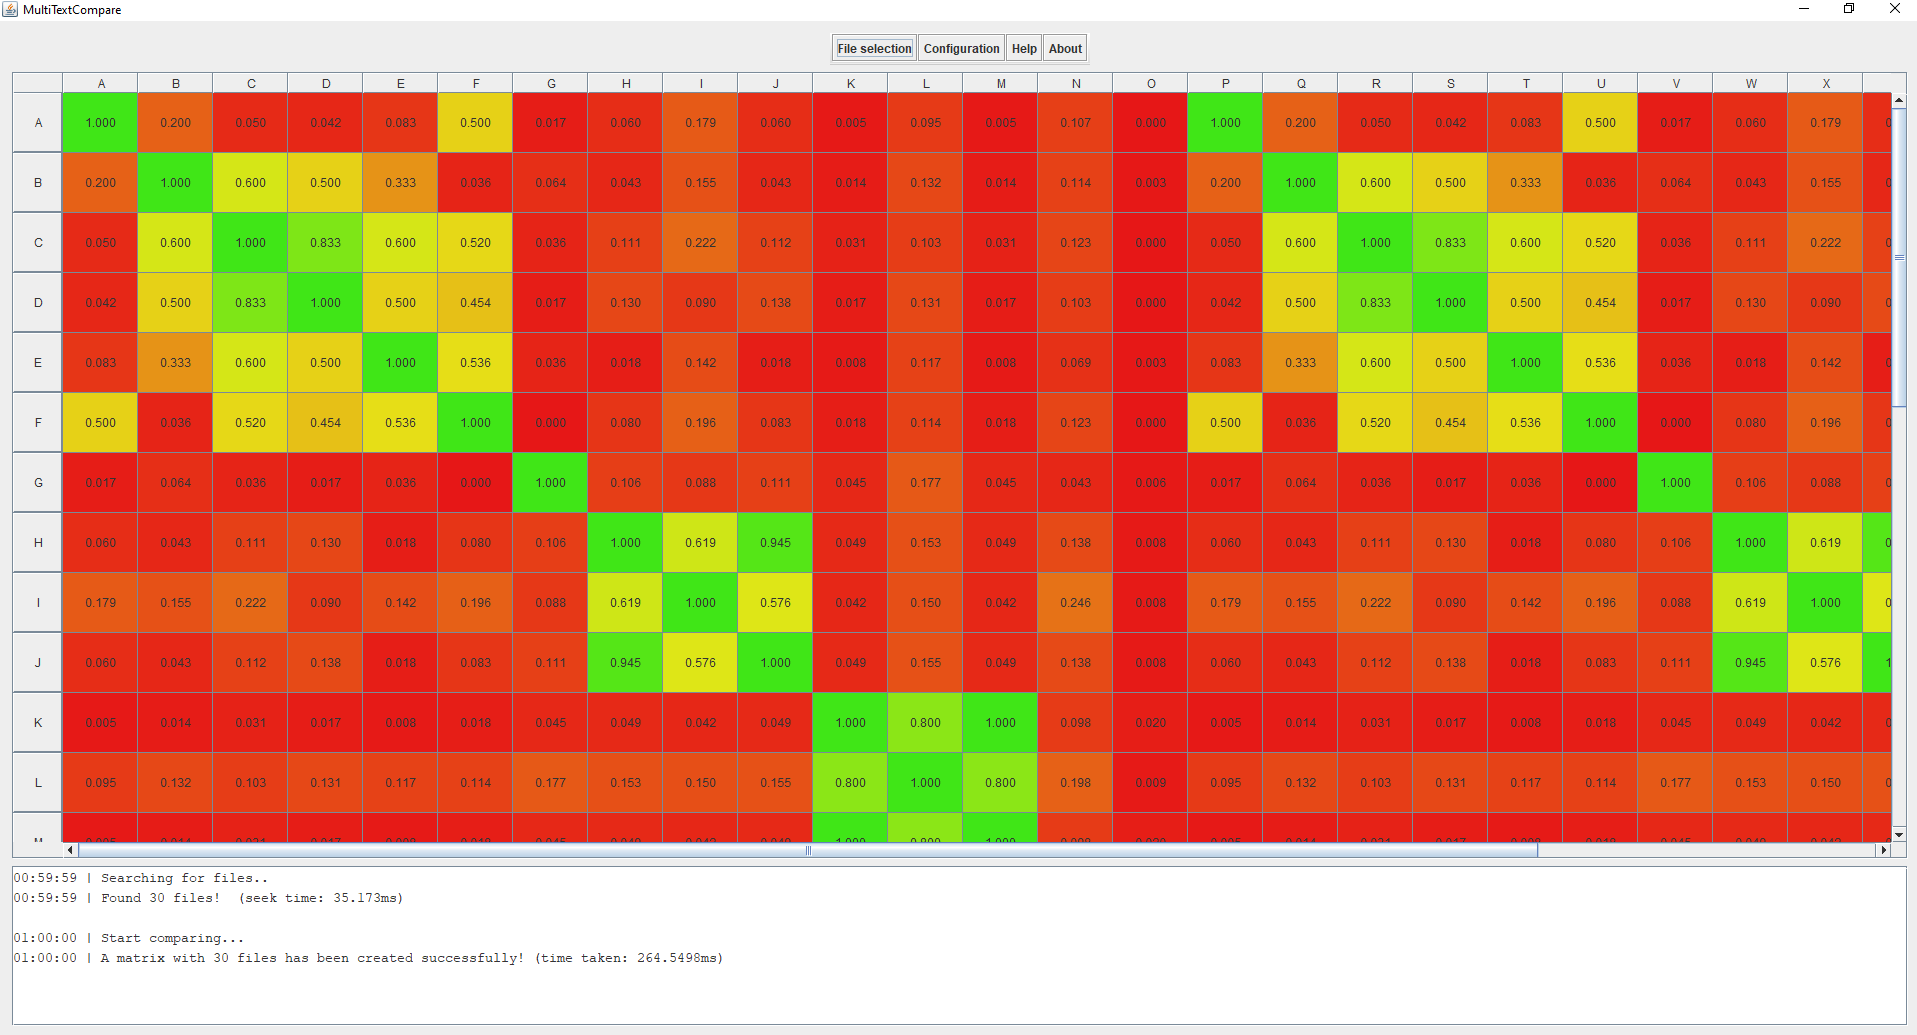
\includegraphics[scale=0.25]{images/matrix V1.png}
    \caption{Ähnlichkeitsmatrix in Version 1.0}
    \label{fig:matrix_v1}
\end{figure}

Zuletzt kann der Benutzer dann auf die einzelnen Zellen der Matrix klicken, um sich die Unterschiede für zwei oder drei Dateien gleichzeitig farbig markieren zu lassen. Dieser Stand der Software wird fortan als Version 1.0 referenziert.

\subsection{Zielsetzung}\label{zielsetzung}
Ziel dieser Arbeit ist es, die Software MultiTextCompare an den nötigen Stellen zu verbessern. Dazu zählen hauptsächlich die Benutzerfreundlichkeit, Laufzeit und die Genauigkeit der Vergleichsalgorithmen.

Dabei gliedert sich die Arbeit in 6 Kapitel: Die theoretischen Grundlagen, die Konzeption der Software, die Implementierung der Verbesserungen, deren Verifikation sowie die Zusammenfassung mit Ausblick.

Die theoretischen Grundlagen sollen zunächst in das Thema des Textvergleichs einleiten. Dafür wird der Begriff der Ähnlichkeit von Zeichenketten diskutiert und anhand von zwei verschiedenen Textvergleichsalgorithmen dargestellt. Darauf folgt eine Übersicht zu den Dateiformaten \acrshort{xml} und \acrshort{json} und eine Vorstellung der speziellen Aspekte in der Programmierung der Software. Dort geht es dann beispielsweise um die Funktionsweise des UI-Toolkits Java Swing und die Implementierung von Nebenläufigkeit in Java.

Das Kapitel zur Konzeption zieht anschließend einen Vergleich zu bereits bestehender Software, deren Vorteilen und ihren Limitationen. Danach werden kurz die besonderen Aspekte für die Entwicklung dargestellt. Darunter liegen bspw. die zu verwendenden Bibliotheken und Tools und die Limitationen der Systeme auf denen die Software lauffähig sein soll. Zuletzt gibt es einen kurzen Überblick über die bestehende Architektur der Software und der Codebase.

In Kapitel 4 geht es hauptsächlich um die durchzuführenden Aufgaben dieser Arbeit. Es wird also konkret die Vorgehensweise bei der Entwicklung erklärt. Dabei soll auch gezeigt werden, durch welche Probleme eine Änderung der Funktionalität notwendig ist, und wie diese Probleme gelöst werden können. Für die Dateiformate \acrshort{xml} und \acrshort{json} sollen zudem eigene Vergleichsalgorithmen entworfen werden, die nun nicht mehr auf reiner Textbasis arbeiten, sondern sich explizit mit den Baumstrukturen der Dokumente auseinandersetzen, um dort einen spezialisierten Vergleich durchführen zu können.

Das fünfte Kapitel beschäftigt sich dann ausführlich mit der Verifikation der in Kapitel 4 durchgeführten Laufzeitoptimierungen und den neuen Vergleichsalgorithmen. Dabei werden die Testsysteme vorgestellt, die Methodik erklärt und die Ergebnisse kritisch evaluiert.

Im letzten Kapitel befindet sich abschließend eine Zusammenfassung der durchgeführten Entwicklungen und der gewonnenen Erkentnisse und ein Ausblick, wie die Software in Zukunft noch weiter verbessert werden könnte.
  % !TeX root = ../BA_LateXVorlage.tex
\section{Grundlagen}
Im folgenden Kapitel werden die theoretischen und technischen Grundlagen erklärt, die für das Verständnis der Funktionsweise von MultiTextCompare notwendig sind.

\subsection{String similarity Algorithmen}\label{String similarity Algorithmen}
Für eine Software, die dazu dient textbasierte Dateien miteinander zu vergleichen ist es essenziell eine Metrik zu finden, die die Ähnlichkeit von Zeichenketten (engl. Strings) bewerten kann. Allerdings ist der Begriff der Ähnlichkeit im allgemeinen Sprachgebrauch ein subjektives Konstrukt. Der Begriff der Gleichheit scheint hingegen auf den ersten Blick etwas greifbarer.
Strings sind gleich, wenn ihre Länge, ihre Zeichen und die Reihenfolge dieser Zeichen gleich sind. In der Sprache existieren allerdings auch Wörter, die bei gleicher Schreibweise unterschiedliche Bedeutungen haben. Wörter sind hierbei im strukturellen Sinne auch nur durch Leerzeichen voneinander getrennte Strings mit Zeichen des zugehörigen Alphabets. Im Deutschen kann z.B. das Wort \glqq einstellen\grqq{} je nach Kontext u.a. die Bedeutung \glqq mit einer Tätigkeit [...] aufhören\grqq{}, \glqq etwas regulieren\grqq{}  und \glqq (jemanden) in ein Arbeitsverhältnis nehmen \grqq{} haben \autocite{dudenEinstellen}, obwohl sich die Schreibweise nicht ändert. Andersherum gibt es Wörter, die anders geschrieben werden und dennoch die gleiche Bedeutung haben. Je nach Kontext können z.B. die Wörter Software, Anwendung und System auf den gleichen Begriff angewandt werden.

Diese Inkonsistenzen sind allerdings schwer messbar und treten zudem bei automatisiert generierten Dateien selten auf, weshalb bei MultiTextCompare auf einen rein strukturellen Vergleich von Strings gesetzt wird. Im Folgenden werden zwei verbreitete Algorithmen für den Vergleich von Strings vorgestellt.

\subsubsection{Longest common subsequence}\label{lcs}

Die \acrfull{lcs} für zwei Strings ist die größte Menge aller Zeichen, die in beiden Strings in gleicher Reihenfolge vorkommen. Diese Menge wird durch Löschung einzelner Zeichen der beiden Strings errechnet, sodass beide Strings nun dieser Menge entsprechen \autocite[]{lcsFirstArticle}. Dadurch dass die Strings nicht gleich lang sein müssen, können Zeichen der Ergebnismenge nicht für beide Strings an den gleichen Indices stehen.

Das folgende Beispiel zeigt zwei unterschiedliche Strings $S_1$ und $S_2$ für die die \acrshort{lcs} berechnet werden soll, wobei unterschiedliche Zeichen in rot markiert sind.

\[ S_1 = \color{black} D \color{red}ie \color{black}s \ ist \ ein \ Text\]
\[ S_2 = D\color{red}a\color{black}s \  ist \  ein  \ \color{red}anderer\color{black} \ Text\]

Die zugehörige Ergebnismenge $M_{LCS}$ ist $ \{Ds \ ist \ ein \ Text\}$. Der \acrshort{lcs} Algorithmus findet Verwendung bei der Erstellung der \acrfull{diff}, einem Verfahren bei dem die Unterschiede zwischen zwei Dateien ermittelt werden. Die Versionskontroll-Software Git, ermittelt bspw. die \acrshort{diff} für verschiedene Versionen der gleichen Datei. Dafür wird grundsätzlich der \acrshort{lcs}-Algorithmus verwendet \autocite{diffLCS}.

Die Implementierung der \acrshort{diff} in der Software MultiTextCompare beruht für zwei Dateien ebenfalls auf dem gleichen Prinzip. Dort entsteht für zwei Dateien $A $ und $B$ genau ein Vergleichsdurchlauf $D_2 = \{A,B\}$, für den alle Zeilen von $A$ und $B$ mittels der \acrshort{lcs} miteinander verglichen werden. Zeichen, die sich in der Ergebnismenge $M_{LCS}$ befinden, werden im \acrfull{ui} als unverändert (weiß) dargestellt, gelöschte und eingefügte Zeichen werden entsprechend rot und grün markiert.
Für drei Dateien $A$, $B$, $C$ wird weiterhin die \acrshort{lcs} verwendet, allerdings entstehen dort 3 Vergleichsdurchläufe $D_3 = \{ \{A,B\}, \{A,C\}, \{B,C\} \}$. Dieses Verhalten wird im Vergleich zu alternativer Software in Kapitel 3.1 genauer beleuchtet. 

Eine weitere interessante Metrik ist die Länge der LCS (LLCS). Diese entspricht für das Beispiel oben $|M_{LCS}| = 15$ und gilt als sinnvolle Quantifizierung der Ähnlichkeit von zwei oder mehr Strings. Als Metrik ist sie auch verwandt zur \textit{Edit Distance}, der minimalen Anzahl an Einfügungen, Löschungen und Änderungen von Zeichen um einen String in einen anderen zu überführen \autocite{llcs}. Im Gegensatz zur Edit Distance beschreibt die \acrshort{llcs} allerdings die Anzahl der \textit{gemeinsamen} Zeichen. Die beiden Begriffe sind also zu einem gewissen Grad komplementär.

% HIER NOCH ETWAS DAZU EINFÜGEN DASS NUR INSERTS UND DELETIONS ERLAUBT SIND ?

Auch die \acrshort{llcs} wird innerhalb von MultiTextCompare verwendet. Durch sie wird im \acrshort{diff}-Prozess festgestellt ob zwei Strings eine Mindestähnlichkeit erfüllen um zu entscheiden, ob gleiche Zeichen noch als gleich geblieben angezeigt werden sollen oder die zwei Strings eine komplette Zeilenlöschung bzw. Zeileneinfügung repräsentieren.

Damit ähnliche, aber verschobene Zeilen miteinander für die \acrshort{diff} verglichen werden können, existiert ein Matcher, der innerhalb der zu vergleichenden Dateien nach ähnlichen Zeilen sucht um diese an den selben Zeilenindex zu schreiben. Für die jeweiligen Strings $S_1, S_2$ zweier nichtleerer Zeilen $Z_1, Z_2$ existiert genau dann ein Match $M$ wenn

\begin{equation}
    \acrshort{llcs}(S_1,S_2) \geq (max(|S_1|, |S_2| ) \cdot x), \ mit \ 0 \leq x \leq 1
    \label{eq:matchat}
\end{equation}

gilt, wobei $x$ ein vom Benutzer einstellbarer Ähnlichkeitsfaktor ist. 


\subsubsection{Levenshtein-Distanz}\label{Levenshtein-Distanz}

Die Levenshtein-Distanz, benannt nach dem russischen Mathematiker Vladimir Levenshtein, ist eine weitere verbreitete Form der Edit Distance. Im Gegensatz zur \acrshort{llcs} beschreibt sie nun tatsächlich die minimale Anzahl an Operationen um Strings ineinander zu überführen und nicht mehr wie ähnlich sich zwei Strings sind. Als kleines Beispiel wird in Abb. \ref{fig:editDist} die Transformation des Wortes \glqq Geschenk\grqq{} in \glqq Gebiet\grqq{} vorgeführt. Ein orangener Knoten symbolisiert eine Änderung und ein roter Knoten steht für eine Löschung und ein dicker, schwarzer Rand kennzeichnet ein unverändertes Zeichen. Dabei ergibt sich für die beiden Strings eine Edit Distance von 5 und ist damit gleich der Anzahl der unterschiedlichen, farbigen Knoten.

\begin{figure}
    %Original
\begin{tikzpicture}[roundnode/.style={circle, draw=black, fill=white, semithick, minimum size=7mm},
currentnode/.style={circle, draw=black, fill=white, very thick, minimum size=7mm}]
\node[roundnode] (g) {G};
\node[roundnode] (e1) [right=of g] {e};
\node[roundnode] (s) [right=of e1] {s};
\node[roundnode] (c) [right=of s] {c};
\node[roundnode] (h) [right=of c] {h};
\node[roundnode] (e2) [right=of h] {e};
\node[roundnode] (n) [right=of e2] {n};
\node[roundnode] (k) [right=of n] {k};

\draw[->] (g.east) -- (e1.west);
\draw[->] (e1.east) -- (s.west);
\draw[->] (s.east) -- (c.west);
\draw[->] (c.east) -- (h.west);
\draw[->] (h.east) -- (e2.west);
\draw[->] (e2.east) -- (n.west);
\draw[->] (n.east) -- (k.west);
\end{tikzpicture}

\begin{tikzpicture}[roundnode/.style={circle, draw=black, fill=white, semithick, minimum size=7mm},
currentnode/.style={circle, draw=black, fill=white, very thick, minimum size=7mm}]
\node[currentnode] (g) {G};
\node[roundnode] (e1) [right=of g] {e};
\node[roundnode] (s) [right=of e1] {s};
\node[roundnode] (c) [right=of s] {c};
\node[roundnode] (h) [right=of c] {h};
\node[roundnode] (e2) [right=of h] {e};
\node[roundnode] (n) [right=of e2] {n};
\node[roundnode] (k) [right=of n] {k};

\draw[->] (g.east) -- (e1.west);
\draw[->] (e1.east) -- (s.west);
\draw[->] (s.east) -- (c.west);
\draw[->] (c.east) -- (h.west);
\draw[->] (h.east) -- (e2.west);
\draw[->] (e2.east) -- (n.west);
\draw[->] (n.east) -- (k.west);
\end{tikzpicture}

\begin{tikzpicture}[roundnode/.style={circle, draw=black, fill=white, semithick, minimum size=7mm},
currentnode/.style={circle, draw=black, fill=white, very thick, minimum size=7mm}]
\node[currentnode] (g) {G};
\node[currentnode] (e1) [right=of g] {e};
\node[roundnode] (s) [right=of e1] {s};
\node[roundnode] (c) [right=of s] {c};
\node[roundnode] (h) [right=of c] {h};
\node[roundnode] (e2) [right=of h] {e};
\node[roundnode] (n) [right=of e2] {n};
\node[roundnode] (k) [right=of n] {k};

\draw[->] (g.east) -- (e1.west);
\draw[->] (e1.east) -- (s.west);
\draw[->] (s.east) -- (c.west);
\draw[->] (c.east) -- (h.west);
\draw[->] (h.east) -- (e2.west);
\draw[->] (e2.east) -- (n.west);
\draw[->] (n.east) -- (k.west);
\end{tikzpicture}

\begin{tikzpicture}[roundnode/.style={circle, draw=black, fill=white, semithick, minimum size=7mm},
currentnode/.style={circle, draw=black, fill=white, very thick, minimum size=7mm},
replacenode/.style={circle, draw=orange, fill=white, very thick, minimum size=7mm}]
\node[currentnode] (g) {G};
\node[currentnode] (e1) [right=of g] {e};
\node[replacenode] (s) [right=of e1] {b};
\node[roundnode] (c) [right=of s] {c};
\node[roundnode] (h) [right=of c] {h};
\node[roundnode] (e2) [right=of h] {e};
\node[roundnode] (n) [right=of e2] {n};
\node[roundnode] (k) [right=of n] {k};

\draw[->] (g.east) -- (e1.west);
\draw[->] (e1.east) -- (s.west);
\draw[->] (s.east) -- (c.west);
\draw[->] (c.east) -- (h.west);
\draw[->] (h.east) -- (e2.west);
\draw[->] (e2.east) -- (n.west);
\draw[->] (n.east) -- (k.west);
\end{tikzpicture}

\begin{tikzpicture}[roundnode/.style={circle, draw=black, fill=white, semithick, minimum size=7mm},
currentnode/.style={circle, draw=black, fill=white, very thick, minimum size=7mm},
replacenode/.style={circle, draw=orange, fill=white, very thick, minimum size=7mm}]
\node[currentnode] (g) {G};
\node[currentnode] (e1) [right=of g] {e};
\node[replacenode] (s) [right=of e1] {b};
\node[replacenode] (c) [right=of s] {i};
\node[roundnode] (h) [right=of c] {h};
\node[roundnode] (e2) [right=of h] {e};
\node[roundnode] (n) [right=of e2] {n};
\node[roundnode] (k) [right=of n] {k};

\draw[->] (g.east) -- (e1.west);
\draw[->] (e1.east) -- (s.west);
\draw[->] (s.east) -- (c.west);
\draw[->] (c.east) -- (h.west);
\draw[->] (h.east) -- (e2.west);
\draw[->] (e2.east) -- (n.west);
\draw[->] (n.east) -- (k.west);
\end{tikzpicture}

\begin{tikzpicture}[roundnode/.style={circle, draw=black, fill=white, semithick, minimum size=7mm},
currentnode/.style={circle, draw=black, fill=white, very thick, minimum size=7mm},
replacenode/.style={circle, draw=orange, fill=white, very thick, minimum size=7mm},
deletenode/.style={circle, draw=red, fill=white, very thick, minimum size=7mm}]
\node[currentnode] (g) {G};
\node[currentnode] (e1) [right=of g] {e};
\node[replacenode] (s) [right=of e1] {b};
\node[replacenode] (c) [right=of s] {i};
\node[deletenode] (h) [right=of c] {h};
\node[roundnode] (e2) [right=of h] {e};
\node[roundnode] (n) [right=of e2] {n};
\node[roundnode] (k) [right=of n] {k};

\draw[->] (g.east) -- (e1.west);
\draw[->] (e1.east) -- (s.west);
\draw[->] (s.east) -- (c.west);
\draw[->] (c.east) -- (h.west);
\draw[->] (h.east) -- (e2.west);
\draw[->] (e2.east) -- (n.west);
\draw[->] (n.east) -- (k.west);
\end{tikzpicture}

\begin{tikzpicture}[roundnode/.style={circle, draw=black, fill=white, semithick, minimum size=7mm},
currentnode/.style={circle, draw=black, fill=white, very thick, minimum size=7mm},
replacenode/.style={circle, draw=orange, fill=white, very thick, minimum size=7mm},
deletenode/.style={circle, draw=red, fill=white, very thick, minimum size=7mm}]
\node[currentnode] (g) {G};
\node[currentnode] (e1) [right=of g] {e};
\node[replacenode] (s) [right=of e1] {b};
\node[replacenode] (c) [right=of s] {i};
\node[currentnode] (e2) [right=of h] {e};
\node[roundnode] (n) [right=of e2] {n};
\node[roundnode] (k) [right=of n] {k};

\draw[->] (g.east) -- (e1.west);
\draw[->] (e1.east) -- (s.west);
\draw[->] (s.east) -- (c.west);
\draw[->] (c.east) -- (e2.west);
\draw[->] (e2.east) -- (n.west);
\draw[->] (n.east) -- (k.west);
\end{tikzpicture}

\begin{tikzpicture}[roundnode/.style={circle, draw=black, fill=white, semithick, minimum size=7mm},
currentnode/.style={circle, draw=black, fill=white, very thick, minimum size=7mm},
replacenode/.style={circle, draw=orange, fill=white, very thick, minimum size=7mm},
deletenode/.style={circle, draw=red, fill=white, very thick, minimum size=7mm}]
\node[currentnode] (g) {G};
\node[currentnode] (e1) [right=of g] {e};
\node[replacenode] (s) [right=of e1] {b};
\node[replacenode] (c) [right=of s] {i};
\node[currentnode] (e2) [right=of h] {e};
\node[replacenode] (n) [right=of e2] {t};
\node[roundnode] (k) [right=of n] {k};

\draw[->] (g.east) -- (e1.west);
\draw[->] (e1.east) -- (s.west);
\draw[->] (s.east) -- (c.west);
\draw[->] (c.east) -- (e2.west);
\draw[->] (e2.east) -- (n.west);
\draw[->] (n.east) -- (k.west);
\end{tikzpicture}

\begin{tikzpicture}[roundnode/.style={circle, draw=black, fill=white, semithick, minimum size=7mm},
currentnode/.style={circle, draw=black, fill=white, very thick, minimum size=7mm},
replacenode/.style={circle, draw=orange, fill=white, very thick, minimum size=7mm},
deletenode/.style={circle, draw=red, fill=white, very thick, minimum size=7mm}]
\node[currentnode] (g) {G};
\node[currentnode] (e1) [right=of g] {e};
\node[replacenode] (s) [right=of e1] {b};
\node[replacenode] (c) [right=of s] {i};
\node[currentnode] (e2) [right=of h] {e};
\node[replacenode] (n) [right=of e2] {t};
\node[deletenode] (k) [right=of n] {k};

\draw[->] (g.east) -- (e1.west);
\draw[->] (e1.east) -- (s.west);
\draw[->] (s.east) -- (c.west);
\draw[->] (c.east) -- (e2.west);
\draw[->] (e2.east) -- (n.west);
\draw[->] (n.east) -- (k.west);
\end{tikzpicture}

\begin{tikzpicture}[roundnode/.style={circle, draw=black, fill=white, semithick, minimum size=7mm},
currentnode/.style={circle, draw=black, fill=white, very thick, minimum size=7mm},
replacenode/.style={circle, draw=orange, fill=white, very thick, minimum size=7mm},
deletenode/.style={circle, draw=red, fill=white, very thick, minimum size=7mm}]
\node[currentnode] (g) {G};
\node[currentnode] (e1) [right=of g] {e};
\node[currentnode] (s) [right=of e1] {b};
\node[currentnode] (c) [right=of s] {i};
\node[currentnode] (e2) [right=of h] {e};
\node[currentnode] (n) [right=of e2] {t};


\draw[->] (g.east) -- (e1.west);
\draw[->] (e1.east) -- (s.west);
\draw[->] (s.east) -- (c.west);
\draw[->] (c.east) -- (e2.west);
\draw[->] (e2.east) -- (n.west);

\end{tikzpicture}
    \caption{Beispiel der String-Transformation}
    \label{fig:editDist}
\end{figure}

Allerdings kann diese Distanz für zwei Strings $S_1$ und $S_2$ auch in ein Ähnlichkeitsmaß überführt werden:

\begin{equation}
    Ähnlichkeit(S_1, S_2) = 1 - \frac{LevenshteinDist(S_1, S_2)}{max(|S_1, S_2|)}
    \label{eq:similarityFunc}
\end{equation}
Für das Beispiel in Abb. \ref{fig:editDist} ergibt sich dann eine Ähnlichkeit von $0,375\%$. 

Diese Funktion wird im MultiTextCompare eingesetzt um die Ähnlichkeit für Dateien prozentual zu quantifizieren. Im \textit{Line Compare}-Modus werden für zwei Dateien A und B Zeile für Zeile die Ähnlichkeiten nach Gleichung (\ref{eq:similarityFunc}) errechnet und mit einem Gewicht multipliziert.

\begin{equation}
    Zeilengewicht(A,B) = \frac{1}{max(|A|,|B|)}
    \label{eq:zeilengewicht}
\end{equation}

Das Gewicht wird wie in Gleichung \ref{eq:zeilengewicht} errechnet, wobei hier die Länge einer Datei ihrer Zeilenanzahl entspricht. Die Gesamtähnlichkeit der beiden Dateien ergibt sich dabei aus der Summe ihrer Teilähnlichkeiten.

Der zweite Vergleichsmodus \textit{Character compare} funktioniert ebenfalls nach Formel (\ref{eq:similarityFunc}), wobei diesmal die zwei Input-Strings die alphabetisch sortierte Konkatenation der Zeichen aller Zeilen aus der jeweiligen Datei sind. Dies hat den Vorteil, dass Dateien mit gleichem, aber verschieden sortiertem oder verschobenem Inhalt immer noch als gleich erkannt werden. Der Nachteil ist, dass es nur für Dateitypen sinnvoll funktioniert, die eine gewisse Dateistruktur aufweisen und ohnehin ähnlich sind. Dadurch, dass alle Zeichen außerhalb ihrer eigentlichen Reihenfolge betrachtet werden, erhöht sich zudem das Risiko für \textit{false positives}, also Dateien die als ähnlich anerkannt werden obwohl ihre Inhalte semantisch klar verschieden sind.

\subsection{Extensible Markup Language}

\acrfull{xml} ist eine vom \textit{World Wide Web Consortium} (W3C) definierte Auszeichnungssprache, die dazu dient hierarchisch angeordnete Daten strukturiert darzustellen. Diese Strukturierung erfolgt in Form eines Baumes. Jedes XML-Dokument enthält genau einen Wurzelknoten, welcher Kindknoten enthalten kann. Diese Kindknoten können ebenfalls beliebig viele Kindknoten aufweisen \autocite[Abs. 2]{xmlSpec}. 

Die Knoten innerhalb des Baumes können außerdem verschiedene Typen aufweisen. Der Wurzelknoten ist vom Typ Element und schließt weitere Elementknoten ein. Neben Elementknoten existieren auch Attribut- und Textknoten, welche  allerdings stets im Kontext eines Elements existieren. Diese Zusammenhänge sind beispielhaft in Abb. \ref{fig:xml_intro} dargestellt, in welcher eine XML-Datei mit einem zugehörigen Baumgraphen abgebildet ist.

\begin{figure}[!htb]
    \centering

\begin{minted}{xml}
<?xml version="1.0" encoding="UTF-8" standalone="yes"?>
<Song>
	<Artist>Deep Purple</Artist>
	<Name album="Machine Head">Smoke on the Water</Name>
	<Year>1972</Year>
	<Genre type="Rock">
		<Subgenre>Hard Rock</Subgenre>
	</Genre>
</Song>
\end{minted}

  
\begin{tikzpicture}[level distance=1.5cm,
  level 1/.style={sibling distance=3.5cm},
  level 2/.style={sibling distance=3cm},
  element/.style={ draw=black!50!green, fill=white, semithick, minimum size=7mm, align=center},
  attribute/.style={ draw=red, fill=white, semithick, minimum size=7mm, align=center},
  textnode/.style={ draw=black, fill=white, semithick, minimum size=7mm, align=center}]
  \node [element]{Song}
    child {node [element]{Artist}
      child {node [textnode]{Deep \\ Purple}}
    }
    child {node [element]{Name}
      child {node [attribute]{Machine \\ Head} edge from parent node[left, color=green!60!red]{album}}
      child {node [textnode]{Smoke on \\ the Water}}
    }
    child {node [element]{Year}
      child {node [textnode]{1972}}
    }
    child {node [element]{Genre}
      child {node [attribute]{Rock} edge from parent node[left, color=green!60!red]{type}}
      child {node [element]{Subgenre}
        child {node [textnode]{Hard Rock}}
      }
    };
\end{tikzpicture}
  \label{fig:xml_tree_intro}

\caption{XML-Datei und zugehöriger Baum}
\label{fig:xml_intro}
\end{figure}

Darüber hinaus existieren noch weitere Knotentypen wie Kommentare oder CDATA-Abschnitte, wobei letztere eine Sonderform des Textknotens sind und auch sonst für Markup reservierte Zeichen erlauben \autocite[Abs. 2.7]{xmlSpec}. 

Zuletzt sollen noch kurz die Begriffe der \textit{Wohlgeformtheit} und der \textit{Validität} eingeführt werden. Ein XML-Dokument ist dann wohlgeformt, wenn alle Regeln gemäß der Definition der W3C in dem Dokument eingehalten werden. Diese beinhalten u.\,a., dass es wie zuvor erwähnt nur ein Wurzelelement gibt oder dass jedes geöffnete Tag <\textit{Elementname}> auch ein schließendes Tag </\textit{Elementname}> besitzt \autocite[Abs. 2.1]{xmlSpec}.

Ein valides XML-Dokument muss wohlgeformt sein, einer Grammatik zugehörig sein und diese auch einhalten. Mögliche Formen dieser Grammatiken sind Dokumenttypdefinitionen (DTD) und XML-Schemadefinitionen (XSD)\autocite[Abs 2.8]{xmlSpec}\autocite[Abs 2.1]{xsdSpec}. 

\subsection{JavaScript Object Notation}

\acrfull{json} ist ein weiteres textbasiertes Datenformat, welches auf einer hierarchischen Datenstruktur basiert und dadurch als Baumstruktur betrachtet werden kann. Es ist dadurch in bestimmten Aspekten ähnlich zu XML, wobei es aber distinkte Unterschiede gibt. 

Jedes JSON-Dokument beginnt mit einem Wurzelknoten, welches anders als in XML keinen eigenen Namen hat und damit ausschließlich Informationen zu den eigenen Kindknoten beinhaltet. Für diese Kindknoten existieren im Wesentlichen 3 verschidene Knoten- bzw. Elementtypen:

\begin{description}
\item[Value-Knoten]
Die einfachste Form in JSON Daten zu speichern, ist in einem einzigen Key-Value Paar. Der Key ist dabei ein auf der aktuellen Ebene eindeutiger Identifier, welcher innerhalb von doppelten Anführungszeichen steht und von einem Doppelpunkt gefolgt wird. Das Value kann ein Integer-, Boolean-, String- oder Null-Wert sein \autocite[]{jsonSpec}. Für Strings besteht die Besonderheit, dass dort das Value auch in doppelten Anführungszeichen stehen muss.
\item[Array-Knoten]
Ein JSON-Array ist eine geordnete Liste an beliebigen Elementtypen, die jeweils durch Kommata getrennt sind \autocite[]{jsonSpec}. Ein Array hat auch genau einen für die Ebene eindeutigen Key und die Value-Elemente werden über ihren Index im Array adressiert. Diese Elementliste beginnt mit einem \glqq $[$ \grqq{} und endet mit einem \break\glqq $]$ \grqq{}.
\item[Objekt-Knoten]
Ein JSON-Objekt wird ebenfalls über einen eindeutigen Key adressiert. Es beinhaltet eine ungeordnete Liste an Elementen, welche wie beim Array durch Kommata getrennt sind. Anders als beim Array ist jedes Element innerhalb eines Objekts ein Key-Value Paar, und wird über den Key adressiert. Die Elemente eines JSON-Objekts sind durch \glqq \{ \grqq{} bzw. \glqq \} \grqq{} begrenzt.
\end{description}

Im Vergleich zu XML fehlt also die Unterstützung für Attribute und Kommentare als Knotentyp. Häufig lassen sich dennoch Informationen aus einer XML-Darstellung in JSON übersetzen. Dies ist hier beispielhaft für die XML-Datei aus Abb. \ref{fig:xml_intro} geschehen. 

\begin{figure}[!htb]
\begin{minted}{json}
{
    "Artist": "Deep Purple",
    "Name": {
       "Album": "Machine Head",
       "Name": "Smoke on the Water"
    },
    "Year": 1972,
    "Genre": {
       "Type": "Rock",
       "Subgenre": ["Hard Rock"]
    }
 }
\end{minted}
\caption{JSON-Datei analog zu Abb. \ref{fig:xml_intro}}
\label{fig:json_intro}
\end{figure}

Analog zu XML existieren die Begriffe der Wohlgeformtheit und Validität auch für JSON. Für valide JSON-Dateien existieren JSON-basierte Schemata gegen die diese Dateien geprüft werden. Außerdem muss eine valide JSON-Datei wohlgeformt sein und darf dadurch keine strukturellen Fehler beinhalten.

\newpage
\subsection{Java}
Java ist eine vielseitige, objektorientierte und weit verbreitete Programmiersprache. Laut \autocite{tiobe} gehört Java auch aktuell noch zu den 3 beliebtesten Programmiersprachen nach C und Python. Im Folgenden werden Java-spezifische Aspekte, die für das Projekt relevant sind, kurz aufgeführt. 

\subsubsection{Verwendete Libraries}

Für die Entwicklung einer Software mit mehreren Funktionen ist es häufig von Vorteil, bereits geschriebenen Code von reputablen Quellen wiederzuverwenden. Im Kontext von Java ist es möglich, fremden Code in Form von Libraries zu verwenden. Zu den zugehörigen Vorteilen gehört zum einen die Zeitersparnis, da der Code nicht neu entwickelt werden muss und zum anderen die Qualität des Codes. Häufig sind Libraries Open-Source, wodurch jeder Entwickler die Möglichkeit hat Fehler zu finden und zu melden oder diese direkt zu beheben. 

Bei der Entwicklung von MultiTextCompare wurden deshalb mehrere Libraries verwendet. 

\paragraph{JDOM}\mbox{}\\
JDOM bietet eine breit aufgestellte API zur Verarbeitung von XML-Dateien. In MultiTextCompare wird JDOM verwendet um XML-Dateien auf Wohlgeformtheit und Validität zu prüfen, um sie bspw. durch Sortierung zu manipulieren und um ihre XML-Strukturbäume für den Vergleich zu nutzen. Für die Validierung enthält JDOM einen Parser, der die Dateien zunächst nur auf Wohlgeformtheit prüft. Je nach Konfiguration ist es auch möglich, die Dateien über DTDs und XSDs zu validieren. Für das Traversieren der Dokumentbäume bzw. des \acrfull{dom} liefert JDOM die Klassen \textit{Element} und \textit{Attribute}. Dabei ist es für jedes Element möglich, dessen Kindelemente und Attribute zu erfragen.

\paragraph{Jackson}\mbox{}\\
Analog zu JDOM und XML bietet Jackson eine API für die Verarbeitung von JSON-Dateien. Die Aufgaben der API im Projekt sind nahezu identisch, wobei hier die Validierung wegfällt. Auch über Jackson lässt sich das \acrshort{dom} erzeugen und navigieren. Dafür existiert die Klasse \textit{JsonNode} mit welcher sich die Kindknoten eines Elements auflisten lassen.

\paragraph{Apache Commons}\mbox{}\\
Apache Commons ist eine Bibliothekssammlung von frei verfügbaren Java-Klassen. Für das Projekt wird die Implementierung der Levenshtein-Distanz, LCS-Länge und \acrshort{diff} innerhalb von \textit{apache.commons.text} verwendet, sowie einige dateibezogene Utility-Methoden aus der Bibliothek \textit{apache.commons.io}.

\subsubsection{Nebenläufigkeit}

Java bietet Entwicklern die Möglichkeit, die Ausführung ihrer Software zu parallelisieren. Konkret passiert das über das Konzept von Threads, also die mögliche Aufteilung von Aufgaben eines zugehörigen Prozesses auf kleinere Teilstücke. Falls keine Parallelisierung stattfindet, existiert pro Prozess genau ein Thread. Prozesse und Threads werden vom Betriebssystem bzw. vom Scheduler des Betriebssystems verwaltet, wobei Java über die Klasse \textit{Thread} Methoden bereitstellt, um Programme aufzuteilen und auf mehrere Threads zu verteilen. Das sog. \textit{Multithreading} hat besonders für Mehrkernprozessoren Vorteile, da die ausgeführte Java-Anwendung so mehrere Prozessorkerne gleichzeitig belasten kann, anstatt alle Aufgaben sequentiell auf einem Prozessorkern abzuarbeiten. Dies kann zu einer erheblichen Verbesserung der Bearbeitungszeit führen.

\subsubsection{Java Swing}

Java Swing ist ein \acrshort{ui}-Toolkit, welches gängige \acrshort{ui}-Komponenten in Form von Java Klassen realisiert und für die Entwicklung zur Verfügung stellt. Dazu gehören u.\,a. Buttons, Textfelder und Labels, die in nahezu jeder Anwendung mit Benutzerinteraktion vorhanden sind. 

Swing ist durch die Vielseitigkeit und Modularität der Komponenten zwar auf der Oberfläche relativ simpel aufgebaut, allerdings gibt es ein paar Besonderheiten im Zusammenhang mit Threads. Für das Event-Handling existiert in Swing der \acrfull{edt}. Wird bspw. ein Button vom Benutzer gedrückt, so wird die dem Button zugehörige Handler-Methode aufgerufen und auf dem \acrshort{edt} ausgeführt \autocite[]{edtDocs}. Für die Ausführungsdauer dieser Handler-Methode ist der \acrshort{edt} dann blockiert und es kann nicht auf weitere Benutzereingaben reagiert werden. 
Um dennoch Methoden mit langer Ausführdauer aus der \acrshort{ui} aufrufen zu können, existiert die Java Klasse \textit{SwingWorker}, die zwei überladene Methoden \textit{doInBackground()} und \textit{done()} zur Verfügung stellt. Für \textit{doInBackground()} wird ein separater Worker-Thread erstellt, auf dem dann die lang andauernden Methoden laufen während der \acrshort{edt} weiterhin auf Benutzereingaben reagiert. Erst sobald der Worker-Thread beendet ist, wird die \textit{done()}-Methode ausgeführt \autocite[]{swingWorkerDocs}.
Ein weiteres, wichtiges Detail ist, dass UI-Komponenten in Swing nicht thread-safe sind. Falls also zwei Threads gleichzeitig auf eine Komponente zugreifen, führt dies zu undefiniertem Verhalten. Dadurch gilt es als \textit{best practice} UI-Komponenten nur über den \acrshort{edt} zu manipulieren \autocite[]{edtDocs}. Im Kontext von SwingWorker, sollten jegliche UI-Zugriffe nur über die \textit{done()}-Methode ausgeführt werden, da diese auf dem \acrshort{edt} ausgeführt wird.
  \section{Konzeption}



\subsection{Vergleich zu bestehender Software}

Im Wesentlichen hat MultiTextCompare zwei zentrale Funktionen. Zum einen den Vergleich beliebig vieler textbasierter Dateien, und zum anderen die Anzeige der \acrshort{diff} für bis zu drei Dateien. Es gibt Anwendungen, die eine prozentuale Ähnlichkeit für zwei Dateien anzeigen können. Jedoch liegt dort der Fokus auf dem semantischen Textvergleich im Sinne der Plagiatserkennung. Wie bereits in \ref{String similarity Algorithmen} erwähnt, arbeitet MultiTextCompare rein zeichenbasiert und reagiert daher nicht auf sprachliche Ähnlichkeiten bei der Ähnlichkeitsbewertung. 

Im Bereich der Diff-Tools existieren häufig Programme, die die Diff für maximal zwei Dateien anzeigen können. Eine Ausnahme ist hierbei die Anwendung \textit{KDiff3}, welche einen Vergleich für drei Dateien zulässt. Um eine Diff für drei Dateien zu erzeugen, muss eine der Dateien als Referenz markiert werden. Für die drei Inputdateien A,B,C mit A als Referenz entstehen dann die Vergleiche $\{A,B\}, \{A,C\}$, während MultiTextCompare keine Datei als Referenz festlegt und jede Datei mit jeder vergleicht. 

Um Unterschiede farbkodiert darzustellen, ist ein Ansatz mit nur zwei Vergleichen zwar für den Benutzer einfacher nachzuvollziehen und zudem performanter als alle drei Vergleiche auszuführen, aber dafür gehen Informationen verloren. Gerade dann, wenn 3 ähnliche Dateien für die Diff ausgewählt werden, kann es interessant sein, die Unterschiede zwischen allen Dateien gleichermaßen zu betrachten.

%Vllt Tabelle mit Farben einfügen%

\subsection{Anforderungen}

Für die Entwicklung der Software MultiTextCompare sind einige funktionale und nicht-funktionale Anforderungen entstanden. Die funktionalen Anforderung wurden bereits größtenteils innerhalb des Einleitungskapitels beschrieben. Zu den nicht-funktionalen Anforderungen gehört der Aspekt, dass die Software speziell für die Laborrechner der Technischen Hochschule Köln entworfen werden soll. Dafür soll Java in der Version 1.7.0\_75 für 32 Bit Systeme verwendet werden. Als IDE soll Eclipse (Release Luna SR2) verwendet werden, um die Code-Basis auch für die Installationen im Labor nahtlos lauffähig zu machen und um nicht auf generierte \acrfull{jar} angewiesen zu sein. Zudem soll die Software primär mit Windows 7 kompatibel sein.

Eine weitere Anforderung ist die einfache Benutzbarkeit. Um dies zu gewährleisten sollen alle notwendigen Funktionen auf den ersten Blick erkennbar, und jegliche Auswahlmöglichkeiten annotiert sein, um dem Benutzer Hilfestellung zu leisten.

\subsection{Architektur}\label{architektur}

Als Architektur wurde auf eine 3-Schichten-Architektur zurückgegriffen. Diese ist grob in Abb. \ref{fig:architektur} als UML-Komponentendiagramm dargestellt. Die Komponenten sind hier als logische Zusammenfassungen von Java Klassen gemeint, wobei jede Komponente aus mindestens einer Java Klasse besteht und genau ein Aufgabengebiet erfüllt. Zusätzlich handelt es sich bei den verwendeten Pfeilen um \textit{<<uses>>} Relationen, wobei die Annotationen zwecks einer besseren Lesbarkeit weggelassen wurden. Aus dem gleichen Grund wurde auf die Darstellung von Interfaces und detailierten Relationen zwischen den Schichten verzichtet.

\begin{figure}[!htb]
    \centering
    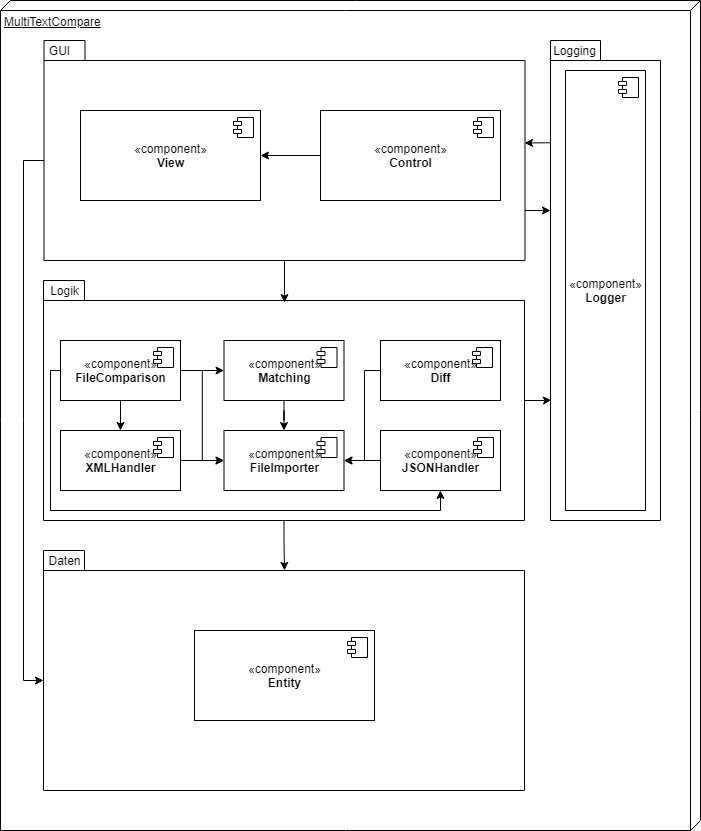
\includegraphics[scale=0.5]{images/Komponenten_MTC_final.png}
    \caption{Übersicht der Architektur}
    \label{fig:architektur}
\end{figure}

In der obersten Schicht liegen alle Java-Klassen, die mit der UI in Verbindung stehen. Dort existiert eine Teilung zwischen Klassen der View-Komponente und denen der Control-Komponente. View-Klassen initialisieren bestimmte UI-Elemente und bestimmen deren Aussehen. Jede View-Klasse, die dynamische Inhalte anzeigen kann, hat eine zugehörige Controller-Klasse für das Event-Handling und Verändern der UI. 

In der Logikschicht befinden sich die Komponenten, die für die Algorithmen und das File-Handling verantwortlich sind. Jede öffentliche Klasse dieser Schicht bietet dabei ein Interface an die GUI-Schicht an. Die Komponente \textit{FileImporter} ist u.\,a. dafür zuständig, die vom Benutzer ausgewählten Dateien zu finden, sie als temporäre Dateien zu klonen und auf die Originaldateien zu mappen. Alle anderen Komponenten greifen auf diese Map zu, um die Dateien weiter zu verarbeiten. Die \emph{FileComparison}-Komponente beherbergt die Vergleichsalgorithmen, die die Werte für die Matrix berechnen. Für Operationen an XML und JSON wie die Filterung oder Sortierung sind die Komponenten XMLHandler bzw. JSONHandler zuständig.

Die Datenschicht ist letztlich eine rein logische Trennung von den anderen Schichten. Da keine Datenbank existiert, gibt es keine Notwendigkeit für CRUD-Komponenten. Die im Diagramm gezeigte Entity-Komponente beherbergt also nur Java Objekte, die für die Speicherung von Daten zur Laufzeit notwendig sind. Dazu gehört bspw. die Klasse \,\textit{IConfigImpl}, die ein Klassenattribut für jede konfigurierbare Einstellung enthält und zur Laufzeit mit dem Inhalt der aktiven Konfigurationsdatei befüllt wird. Jede Entitätsklasse besitzt ebenfalls ein zugehöriges Interface, welches die \emph{Getter} und \emph{Setter} an höhere Schichten übergibt.

Die Logging-Komponente existierte zwar in Version 1.0 noch nicht, da sie aber die einzige architektonische Änderung während der Bearbeitung dieser Arbeit ist, wird sie hier bereits aufgeführt. Sowohl Komponenten aus der Logik-Schicht als auch aus der GUI-Schicht, können Fehler loggen. Diese Fehler werden in der UI dargestellt, falls das entsprechende Log-Level vom Benutzer gesetzt ist. Die genauere Funktionsweise wird in Kapitel \ref{logging} beschrieben. Informationen zu den einzelnen Klassen, Interfaces und Methoden können als Javadoc direkt über MultiTextCompare im Browser geöffnet werden.



  \section{Implementierung}\label{implementierung}

In diesem Kapitel werden die in \ref{zielsetzung} geplanten Verbesserungen an MultiTextCompare durchgeführt und dargestellt. Angegebene Codestücke sind zwecks Lesbarkeit teilweise auf die relevantesten Zeilen gekürzt.

\subsection{Verbesserung des Zeilenmatchings}\label{verbesserungMatching}

Textbasierte Dateien können inhaltlich identisch sein, ohne dass sie exakt gleich aussehen. Sind zwei Dateien inhaltlich identisch aber um eine Zeile verschoben, würden sie von der Software als sehr unterschiedlich bewertet werden. Daher existiert die Matching-Komponente, die sicherstellt dass gleiche oder ähnliche Zeilen erkannt werden, und in der Diff-Anzeige im gleichen Zeilenindex stehen.

Diese Eigenschaft ist daher unerlässlich für den Diff-Prozess innerhalb der Software. Im Kontext der Laufzeit, ist sie aber sehr kostspielig weshalb Maßnahmen notwendig sind, um diese zu senken. Dafür wird hier zunächst die ursprüngliche Funktionsweise in Version 1.0 zusammengefasst dargestellt.

\subsubsection{Optimierung des Matching-Algorithmus}

Das Matching kann in zwei Teilprobleme zerlegt werden. Auf der einen Seite existiert die Matcherkennung, bei der festgelegt wird ob zwei Zeilen überhaupt gematcht werden können. Auf der anderen Seite gibt es noch das Alignment, also die Sicherstellung davon, dass alle Zeilen nach dem Matching korrekt dargestellt werden können. Im Folgenden wird nur auf den ersten Aspekt eingegangen, da dieser die hauptsächliche Funktionalität darstellt.

Um für zwei Dateien A und B alle Matches zu ermitteln, wird zunächst die Datei mit weniger Zeilen als Referenzdatei festgelegt. Dies sei ab jetzt Datei A. In Version 1.0 wurde für jede Zeile von A jede Zeile von B nach einem Match durchsucht. Die Kriterien für ein Match waren dabei, dass sich die Zeilen nach Gleichung (\ref{eq:matchat}) ähnlich genug sind und dass keine der infrage kommenden Zeilen bereits gematcht wurde. Zudem sind Matches \glqq über Kreuz\grqq{} ausgeschlossen. Das heißt, dass die Matchindices für ein potenzielles Match immer größer sein mussten, als die des letzten erfassten Match. Der zugehörige Code ist in Codeabschnitt \ref{code:matchingV1} dargestellt.

\begin{listing}
\begin{minted}
[
frame=lines,
framesep=2mm,
baselinestretch=1.2,
bgcolor=white,
fontsize=\footnotesize,
linenos
]{java}

String ref = "", comp = "";
int lastMatchedIndex = 0;
// Schaue für jede Zeile der linken Datei
for (int i = 0; i < lineCountLeft; i++) {
	reference = leftFile.get(i);
	// ob es in der rechten Datei ein Match gibt
	for (int j = 0; j < lineCountRight; j++) {
		comp = rightFile.get(j);
		if (matches(reference, comp) // falls Zeilen ähnlich genug
				&& j >= lastMatchedIndex // falls Match nicht über Kreuz
				&& notMatchedYet(i, j)) { // falls noch nicht gematcht
			lastMatchedIndex = j;
			// Speichere Match
			matches.add(new IMatchImpl(i, j, reference, comp));
			// Gehe in die nächste Zeile der Referenzdatei
			break;
		}

	}
}
\end{minted}
\caption{Matching in V1.0}
\label{code:matchingV1}
\end{listing}


Besonders ausschlaggebend für die Laufzeit ist dabei die Feststellung der Ähnlichkeit. Für eine Optimierung sollte die Anzahl dieser Feststellungen also, wo möglich, reduziert werden.

Für den Fall, dass in beiden Dateien kein einziges Match existiert, würde jede Zeile von A mit jeder Zeile von B verglichen werden. Dieses Szenario enthält die größtmögliche Anzahl an Vergleichen und stellt daher den worst case dar. Um hier die Laufzeit zu verbessern, wird ein \textit{Lookahead}-Limit eingeführt. Das bedeutet, dass für jede Zeile der Referenzdatei $A_i$ eine maximale Suchreichweite abhängig vom aktuellen Zeilenindex $i$ festgelegt wird.
Als Beispiel würde eine Zeile $A_5$ mit einem Lookahead-Wert von 10 mit jeder Zeile $B_{0...15}$ verglichen werden sofern kein Match für $B_{0...15}$ existiert und Datei B mindestens 15 Zeilen lang ist. Ist Datei B kürzer, so werden alle Zeilen bis zum Dateiende verglichen. 

Auch wenn Matches existieren, kann ein solches Lookehead-Limit Vorteile haben. Für größere Dateien kann es passieren, dass ein Match erst 50-100 Zeilen nach dem letzten gefunden wird. Dies führt dann zu genauso vielen Leerzeilen im Alignment-Prozess, was die Lesbarkeit für den Benutzer beeinträchtigen kann. Da die Eingabedateien vor dem Vergleichen nicht bekannt sind, wird dem Benutzer die Möglichkeit gegeben, den Schwellwert selbst nach Bedarf anzupassen.

Eine weitere Auffäligkeit im Quellcode-Abschnitt \ref{code:matchingV1} ist, dass die Indexvariable j, unabhängig davon ob ein Match gefunden wird oder nicht, immer bei 0 anfängt. Dabei würde es genügen, wenn nach einem Match $M_{i,j}$ der Vergleich erst bei $i = i + 1$ und $j = j + 1$ fortgesetzt werden würde. So müsste auch nicht mehr geprüft werden ob ein Match über Kreuz ist oder ob es bereits ein Match mit den aktuellen Indices gibt. Diese Optimierungen sind im Quellcode \ref{code:lookahead} dargestellt

%TODO: PERFORMANCE UNTERSCHIED BESCHREIBEN%

\begin{listing}[!h]
\begin{minted}
[
frame=lines,
framesep=2mm,
baselinestretch=1.2,
bgcolor=white,
fontsize=\footnotesize,
linenos
]{java}

String ref = "", comp = "";
int lowestPossibleIndex = 0;
// Schaue für jede Zeile der linken Datei
for (int i = 0; i < lineCountLeft; i++) {
	reference = leftFile.get(i);
	int maxSearchIndex = i + LOOKAHEAD + 1;
	if (maxSearchIndex > lineCountRight) {
		maxSearchIndex = lineCountRight;
        }
	// ob es in der rechten Datei ein Match gibt
	for (int j = lowestPossibleIndex; j < maxSearchIndex; j++) {
		comp = rightFile.get(j);
		if (matches(reference, comp)) { // falls Zeilen ähnlich genug
			lowestPossibleIndex = j + 1;
			// Speichere Match
			matches.add(new IMatchImpl(i, j, reference, comp));
			// Gehe in die nächste Zeile der Referenzdatei
			break;
		}
	}
}
\end{minted}
\caption{Aktualisiertes Matching mit Lookahead}
\label{code:lookahead}
\end{listing}

\subsubsection{Verbesserung der Funktionsweise}\label{bestMatch}

Trotz Optimierung gibt es noch einen weiteren Aspekt der verbessert werden kann. Aktuell wird die Suche nach Matches nach dem ersten Match beendet. So entstehen Situationen, bei denen mehrere ähnliche Zeilen nah beieinander existieren und ein Match der ersten möglichen Zeile nicht die beste Option wäre.

\begin{figure}
\centering
\begin{subfigure}{.45\textwidth}
  \begin{minted}{json}
{
  "phones" : [ {
	  "brand": "Apple",
	  "name": "IPhone 12"
  },
  {
      "brand": "Apple",
	  "name": "IPhone 13"
  } ]
}
  \end{minted}
  \caption{Beispiel-JSON 1}
  \label{fig:sub1}
\end{subfigure}
\begin{subfigure}{.45\textwidth}
\begin{minted}[stripnl=false]{json}
{
  "phones" : [ {
	  "brand": "Apple",
	  "name": "IPhone 13"
  } ]
}




\end{minted}
  \caption{Beispiel-JSON 2}
  \label{fig:sub2}
\end{subfigure}
\caption{Zwei ähnliche JSON-Dateien}
\label{fig:bestMatchJSON}
\end{figure}

In Abb. \ref{fig:bestMatchJSON} sind zwei JSON-Dateien abgebildet, bei denen dieses Szenario zutrifft. In der Standardeinstellung würden, bis auf die schließenden Klammern, keine Zeilen der zweiten Datei verschoben werden obwohl in Datei 1 ein identischer Eintrag existiert. Zwar könnte der Wert für $x$ aus Gleichung (\ref{eq:matchat}) auf 1 erhöht werden, allerdings würden dadurch nicht-identische aber ähnliche Zeilen für das Matching ignoriert werden falls die Dateien weitere Einträge hätten.

Die Lösung für dieses Problems wird durch einen \textit{Best-Match} Algorithmus gelöst. Innerhalb des Lookahead-Limits werden alle potenziellen Matches in einer zusätzlichen Liste gesammelt. Mit jedem potenziellen Match wird zusätzlich die \acrshort{llcs} mitgespeichert. Nachdem alle nötigen Zeilen verglichen wurden, wird die Kandidatenliste nach der durch die maximale Länge der verglichenen Strings geteilten LLCS sortiert und das Match verwendet, welches dort den höchsten Wert besitzt. Diese Normierung führt u.\,a. dazu, dass ähnlichere Matches trotz gleicher \acrshort{llcs} bevorzugt werden. Ein Beispiel dafür wäre der Vergleich der Zeilenpaare (\emph{Kunde}, \emph{Kunden}) und (\emph{Kunde}, \emph{Kundennummer}), bei denen die LCS für beide Paare 5 ist, aber die Edit-Distance für das zweite Paar mit 7 deutlich größer ausfällt als die des ersten Paares mit Distanz 1. Dadurch ergäbe sich für Paar 1 ein normierter Ähnlichkeitswert von ca. 0,83 und für Paar 2 ein Wert von nur 0,42, weswegen Paar 1 als Match bevorzugt werden würde. Sollte dieser Wert für zwei potenzielle Matches gleich sein, wird danach entschieden ob eins der Matches direkt auf ein vorangegangenes Match folgt, um möglichst nach verschobenen Blöcken zu suchen. Existiert kein direkter Vorgänger und der Ähnlichkeitswert ist gleich, wird das Match mit geringerem Index verwendet. Das Ergebnis innerhalb der Software ist in Abb. \ref{fig:bestMatchResult} dargestellt. Nun werden alle verfügbaren Zeilen der rechten Datei auch in der linken Datei als existent dargestellt. Das Ergebnis zeigt jedoch auch eine Limitation des Verfahrens. Da es nicht auf die Syntax der unterliegenden Dateiformate eingeht, kann nicht darauf geachtet werden ob ganze Objekte oder Array-Einträge verschoben wurden. Für den hier beschriebenen Fall führt diese Limitation wiederum zu keinen Abzügen in der Genauigkeit bei der Bewertung durch den \emph{Line Compare}-Vergleichsmodus.

\begin{figure}[]
    \centering
    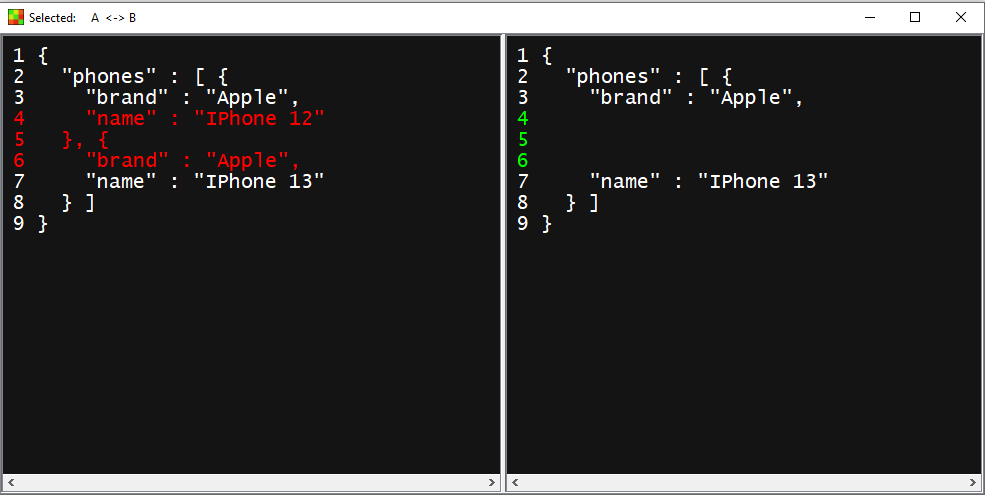
\includegraphics[width=\textwidth]{images/Best Match updated.png}
    \caption{Resultat des Best-Match Verfahrens}
    \label{fig:bestMatchResult}
\end{figure}

\newpage
\subsection{Überarbeitung der Vergleichsalgorithmen}

Das ausschlaggebende Feature der Software ist ihre Ähnlichkeitsmatrix. Diese wurde bereits in der Einleitung kurz erwähnt. Auch die Funktionsweisen der beiden Vergleichsalgorithmen \textit{Line Compare} und \textit{Character Compare} wurden bereits oberflächlich behandelt. Dieses Unterkapitel behandelt nun die Überarbeitung des Modus Line Compare und die Einführung zweier neuer Vergleichsmodi, die sich in ihrer Funktionsweise stark von den bisherigen Algorithmen unterscheiden.

\subsubsection{Zeilenweiser Vergleich regulärer Textdateien}

Line Compare war der erste Vergleichsmodus der Software. Da zum Zeitpunkt der Entwicklung noch keine Matching-Komponente existierte, arbeitete der Vergleichsmodus nicht mehr optimal sobald ähnliche Zeilen leicht verschoben waren. Das Ziel ist nun die Einbettung der Matching-Komponente in den regulären Textvergleich um Dateien, die dem Benutzer in der Diff-Anzeige als ähnlich angezeigt werden würden, auch mit einer höheren Genauigkeit für den Vergleich bewerten zu können.

Alle Vergleiche basieren auf den von der Komponente \emph{FileImporter} erstellten temporären Dateien. Diese sind notwendig um die vom Benutzer ausgewählten Originaldateien bei einer Normierung, also zum Beispiel einer Entfernung aller Leerzeichen, nicht zu verändern. Des Weiteren wurde explizit für den Line Compare Modus ein weiteres Set an temporären Dateien erstellt, bei denen nach jedem Wort ein Zeilenumbruch eingefügt wurde. Als Wort galt eine beliebige Zeichenkette gefolgt von einem Leerzeichen.  

Dieser Prozess sollte eigentlich dazu dienen, um die Genauigkeit des Vergleichs leicht zu verbessern, wobei dies nur für Dateien funktioniert, die ohnehin ähnliche Zeileneinträge in der gleichen Reihenfolge besitzen.

Um die Matching-Komponente in den Vergleich einzubinden, muss zunächst ihre Schnittstelle angepasst werden. Aktuell hat die Matching-Methode \textit{matchLines()} nämlich noch den Rückgabetyp void, denn ihre Erzeugnisse waren bisher immer neue temporäre Dateien im Dateisystem auf die andere Komponenten zugreifen konnten. Um IO-Zugriffe zwecks Laufzeit zu minimieren, erstellt die Methode diese temporären Dateien nicht falls sie für den Vergleich aufgerufen wird. Stattdessen werden die gematchten Zeilen als ein \textit{Object}-Array zurückgegeben. So kann der Rest des Vergleichsalgorithmus unverändert bleiben. Das heißt, dass Zeilen des gleichen Index nach dem in Abschnitt \ref{Levenshtein-Distanz} beschriebenen Verfahren bewertet werden. Sind die beiden zu vergleichenden Dateien nicht gleich lang, wird die kürzere Datei mit Leerzeilen aufgefüllt. Das Ergebnis ist ein zeilenbasierter Vergleichsalgorithmus, der nun verschobene Zeilen erkennen und genauer bewerten kann. Gleichzeitig profitiert er von den in Kapitel \ref{verbesserungMatching} durchgeführen Verbesserungen.

\subsubsection{Vergleich von XML-Dateien}\label{xmlChapter}

\paragraph{Erweiterung der Element-Sortierung}\mbox{}\label{xmlSortierung}

In Version 1.0 besteht bereits die Möglichkeit, die Strukturbäume von XML-Dateien nach ihren Element-Namen und Attribut-Namen zu sortieren. Die Sortierung der Attribute ist insofern eindeutig, als dass ein Attributname pro Element immer einzigartig sein muss. Für Elemente gibt es allerdings keine solche Regel. Elemente, die den gleichen Namen haben und auf der gleichen Ebene innerhalb des Baumgraphen liegen, können als Liste interpretiert werden. 

Vergleichsoperationen wie Line Compare und die Berechnung der Diff würden davon profitieren, wenn XML-Dateien eindeutig sortiert werden könnten, da sie zeilenbasiert operieren. Wenn ähnliche Zeilen in der gleichen Reihenfolge vorliegen, können sie zusätzlich durch das Zeilenmatching erkannt werden. Da weder durch die XML-Spezifikation noch durch die JDOM-API eine Sortierreihenfolge vorgeschrieben wird, wird im Folgenden eine eigene Reihenfolge festgelegt. Diese Priorisierung bezieht sich auf den Vergleich von zwei Elementen:

\newpage
\begin{enumerate}
    \item Elementname
    \item Attributname
    \item Attributwert
    \item Textinhalt
\end{enumerate}

Die Implementierung erfolgt über die Schnittstelle \emph{java.util.Comparator} und das Überschreiben ihrer \textit{compare()}-Methode. Diese gibt einen Integer-Wert zurück mit Hilfe dessen zwei Strings lexikographisch als kleiner, größer oder gleich bewertet werden können. Diese Bewertung wird durch die von JDOM breitgestellte Methode \textit{sortChildren()} ausgewertet, um die Elemente strukturerhaltend zu sortieren.

Sind die Elementnamen identisch, werden die Attribute untersucht. Da Elemente beliebig viele Attribute haben können, werden zunächst nur so viele Attribute verglichen, wie in der kürzesten Attributliste vorhanden sind. Dabei werden erst die Attributnamen verglichen und dann die Werte. Dafür ist vorausgesetzt, dass die Attribute vorher bereits sortiert wurden. Sind die bisher betrachteten Attribute sowohl im Namen als auch im Wert identisch, entscheidet die Anzahl der Attribute. Mehr Attribute werden dabei als größer eingestuft. Bei gleicher Attributzahl werden letztlich noch die Textknoten der Elemente miteinander verglichen. Falls alle dieser Kriterien für die beiden Elemente identisch sind, wird das Verfahren in gleicher Reihenfolge rekursiv für alle Kindknoten der beiden infrage stehenden Elemente durchgeführt, bis ein Unterschied festgestellt wird. Bei Gleichheit der Elemente wird nichts verändert.

\paragraph{Struktureller Vergleich von XML-Dateien}\mbox{}

Im Vorfeld wurden bereits Limitationen der vorhandenen Vergleichsalgorithmen diskutiert. Weder der zeilen- noch der zeichenbasierte Vergleichsansatz kann für Dateien, die einer gewissen Struktur unterliegen zuverlässig für akkurate Ergebnisse sorgen. Aus diesem Grund wird im Folgenden ein Vergleichsalgorithmus entworfen und implementiert, der XML-Dateien auf Basis der Baumstruktur vergleicht.

Verglichen werden sollen dabei die Element-, Attribut-, Text-, CDATA- und Kommentarknoten, wobei letztere optional sind und durch einen Konfigurationsparameter vom Vergleich ausgeschlossen werden können. Ausschlaggebend für den Vergleich sind allerdings die Elementknoten, da jeder der zuvor genannten Knotentypen ein zugehöriges Elternelement hat. Die einzige Ausnahme ist der Wurzelknoten, wobei dieser vom Vergleich ausgenommen ist. Um \emph{false positives} zu vermeiden werden zwei Elemente nur miteinander verglichen werden, wenn ihre Namen identisch sind.

Durch diesen verschiedenen Ansatz, kann das alte Bewertungssystem für die Ähnlichkeit über die LCS oder die Levenshtein-Distanz hier nicht verwendet werden. Stattdessen wird für den strukturellen Vergleich ein Ähnlichkeitsmaß auf Basis der Baumstruktur eingeführt. In Abb. \ref{fig:ähnlichkeitBaum} ist ein Beispielbaum dargestellt, für den die Gewichte der Knoten an der Kante zum Elternelement annotiert sind. Für eine sinnvolle Bewertung wird hierbei davon ausgegangen, dass innerhalb der zu vergleichenden XML-Dateien wichtige Informationen nah am Wurzelelement liegen. Zunächst wird geschaut, wieviele Elemente $n$ innerhalb der ersten Ebene liegen. Jedes dieser Elemente geht mit einem Gewicht von \( \frac{1}{n} \) in den Gesamtwert der Ähnlichkeit ein. Gleichzeitig wirkt dieses Gewicht als ein Budget für dessen Kindelemente. Im Beispiel hat Knoten 2 ein Gewicht von \( \frac{1}{3} \), welches gleichmäßig auf die Kindknoten verteilt wird. Die beiden Kindknoten 5 und 6 haben also im Kontext von Knoten 2 ein Gewicht von \( \frac{1}{2} \). Das Gewicht eines Knotens für die Gesamtähnlichkeit wird berechnet aus dem Produkt aller Kantengewichte $f(V_1,V_2)$ auf dem Weg zwischen der Wurzel und genau diesem Knoten. Dadurch ergibt sich für Knoten 5 bspw. ein Gesamtgewicht von
\[ f(1,2) \cdot f(2,5) = \frac{1}{3} \cdot \frac{1}{2} = \frac{1}{6}\]
\begin{figure}
    \centering
    \input{Graphs/xmlBaumÄhnlichkeit}
    \caption{Gewichtung von Elementknoten für strukturellen Vergleich}
    \label{fig:ähnlichkeitBaum}
\end{figure}

Um diese Gewichte einzusetzen, muss noch definiert werden wodurch zwei Knoten ähnlich sind. Dafür wird bei den Kindknoten der Elemente zwischen textuellem Inhalt, Attributen und Kommentaren unterschieden. Falls Kommentare ignoriert werden sollen oder keine Kommentare präsent sind, sind einzig der Text und die Attribute zu bewerten. Sollten auch keine Attribute existieren, zählt nur der Textinhalt bzw. sollte kein Textinhalt existieren, zählen nur die Attribute. Der Textinhalt schließt reine Textknoten und CDATA-Knoten ein, da JDOM hier auch keine explizite Unterscheidung macht und sie häufig den gleichen Zweck erfüllen. Falls Elemente keinerlei Kindknoten haben, sind sie identisch. Wie Abb. \ref{fig:elementähnlichkeit} zeigt, wird jeder dieser Knoten, sofern er existiert, gleichwertig gewichtet.

\begin{figure}
    \centering
    \input{Graphs/xmlElementÄhnlichkeit}
    \caption{Beispielhafte Gewichtung eines Elementinhalts für XML}
    \label{fig:elementähnlichkeit}
\end{figure}

Letztlich muss noch sichergestellt werden, dass das Verfahren symmetrisch ist, also die Reihenfolge der verglichenen Bäume nicht das Ergebnis beeinflusst. Ein Beispiel wäre, wenn der Baum aus Abb. \ref{fig:ähnlichkeitBaum} mit einem Baum verglichen werden würde, der auf Ebene 1 vier Knoten besitzt. In diesem Fall würde die maximale Anzahl an Knoten auf der Ebene entscheidend sein, also läge die maximale Ähnlichkeit der Graphen unabhängig vom Inhalt bei \( \frac{3}{4} \). In jeder Situation bei der unterschiedliche Anzahlen an Einträgen existieren können, wird die gemeinsame Anzahl an gleichen Einträgen durch die maximal verfügbare Anzahl geteilt.  

Implementiert wird dieses Konzept indem zunächst die Wurzelknoten der beiden zu vergleichenden Dateien eingelesen werden, wobei einer der Knoten als Referenzknoten festgelegt wird. Dabei ist nicht wichtig welcher der Knoten die Referenz ist, da in XML das Tauschen von Knoten mit gleichem Elternknoten erlaubt ist. Um diesen Vergleichsmodus anwenden zu können, müssen die jeweiligen XML-Dateien wohlgeformt sein, da ansonsten ein Traversieren der Dokumentbäume nicht möglich ist.

Bei vorliegender Wohlgeformtheit wird zunächst für alle Kindknoten der Referenzwurzel, wie in Quellcode \ref{code:knotenMatching} gezeigt, der aktuelle Knotenname in einer Liste gespeichert. Beim ersten Vorkommen dieses Namens werden alle Elemente mit diesem Namen in einer jeweiligen Liste für Referenzknoten (matchingRef) und Vergleichsknoten (matchingComp) gespeichert. Die Methode \emph{getElementCount()} zählt wie oft ein Elementname in einer Liste vorkommt und sorgt dadurch dafür, dass Elementlisten nicht doppelt eingefügt werden.

\begin{listing}[!h]
\begin{minted}
[
frame=lines,
framesep=2mm,
baselinestretch=1.2,
bgcolor=white,
fontsize=\footnotesize,
linenos
]{java}
        List<Element> matchingRef = new ArrayList<Element>();
        List<Element> matchingComp = new ArrayList<Element>();
        List<Element> refFirstLevelChildren = rootRef.getChildren();
        List<String> refElementNames = new ArrayList<String>();
	for (int i = 0; i < refFirstLevelChildren.size(); i++) {
		Element currentRef = refFirstLevelChildren.get(i);
		String currentRefName = currentRef.getName();
		refElementNames.add(currentRefName);
		if (getElementCount(refElementNames, currentRefName) == 1) {
			matchingRef.addAll(rootRef
					.getChildren(currentRefName));
			matchingComp.addAll(rootComp
					.getChildren(currentRefName));
		}
	}
\end{minted}


\caption{Suche nach gleichnamigen Knoten auf gleicher Ebene}
\label{code:knotenMatching}
\end{listing}\newpage

Da die Matching-Komponente für den strukturellen Vergleich nicht eingesetzt werden kann, muss an dieser Stelle noch ein Mechanismus eingeführt werden um gleiche Listeneinträge zu finden und zu vergleichen. Restliche Listeneinträge können dann noch nach ihrem Index geordnet verglichen werden. Allerdings ist es mit JDOM nicht direkt möglich festzustellen ob zwei Elemente tatsächlich gleich sind ohne alle ihre Kindknoten zu betrachten. Die \emph{equals}()-Methode für die Klasse \emph{Element} prüft nicht auf die inhaltliche Ähnlichkeit sondern ob die Referenz zweier Objekte gleich ist. Dadurch, dass eine rekursive Prüfung aller Kindelemente sehr aufwändig sein kann, wird, wie in Quellcode \ref{code:identischeElemente} gezeigt, mit der Klasse \emph{XMLOutputter} von JDOM gearbeitet. Mit ihr ist es nämlich möglich ein Element als String darzustellen. Da die \emph{equals}()-Methode für Strings \emph{true} zurück gibt sobald die verglichenen Zeichensequenzen identisch sind, kann man auf diese Weise die Gleichheit zweier Objekte feststellen. Um identische Elemente vom rekursiven Vergleich auszuschließen, werden diese durch den Wert \emph{null} ersetzt um sie als bereits bewertet zu kennzeichnen. Nachdem alle verfügbaren Elementknoten miteinander auf Gleichheit untersucht wurden, werden gefundenen null-Werte durch eine Hilfsmethode \emph{clearNullValues}() aus den Listen gestrichen. 

\begin{listing}[!tb]
\begin{minted}
[
frame=lines,
framesep=2mm,
baselinestretch=1.2,
bgcolor=white,
fontsize=\footnotesize,
linenos
]{java}
        for (int i = 0; i < matchingRef.size(); i++) {
		Element currentRef = matchingRef.get(i);
		for (int j = 0; j < matchingComp.size(); j++) {
			Element currentComp = matchingComp.get(j);
			if (currentComp == null) {
			    continue;
			}
			XMLOutputter xmlOut = new XMLOutputter();
			String refString = xmlOut.outputString(currentRef);
			String compString = xmlOut.outputString(currentComp);
			boolean equals = refString.equals(compString);
			if (equals) {
			    similarity.add(currentLevelWeight);
			    matchingRef.set(i, null);
			    matchingComp.set(j, null);
			    break;
			}
		}
	}
	matchingRef = clearNullValues(matchingRef);
	matchingComp = clearNullValues(matchingComp);
\end{minted}
\caption{Suche nach identischen Knoten auf gleicher Ebene}
\label{code:identischeElemente}
\end{listing}

Für die restlichen Elementknoten werden noch die Inhalte verglichen. Der Vergleich von Textknoten, Attributwerten und Kommentaren basiert auf der Levenshtein-Distanz bzw. der Gleichung (\ref{eq:similarityFunc}), da es sich hierbei um reguläre Texte handelt. Bei Attributen werden, wie bei Elementen, nur Attribute mit identischem Namen verglichen. Kommentare werden, falls sie zu mehreren für ein Element existieren, in ihrer originalen Reihenfolge betrachtet. 

Alle aus Quellcode \ref{code:identischeElemente} übrig gebliebenen Knoten in der Liste \emph{matchingRef} bzw. \emph{matchingComp} werden in ihrer bestehenden Reihenfolge rekursiv miteinander verglichen. Falls die Listen unterschiedlich lang sind, werden so viele Elemente verglichen wie sie in der kürzeren Liste vorhanden sind, da die restlichen Knoten ohnehin nicht in beiden Bäumen vorhanden sein können.

\newpage\subsubsection{Vergleich von JSON-Dateien}

\paragraph{Erweiterung der Sortierung}\mbox{}

Anders als bei XML, existiert für JSON die Möglichkeit Elemente nach ihren Namen eindeutig zu sortieren da die Namen bzw. Keys innerhalb einer Ebene eindeutig sind. Innerhalb der Container-Elemente Array und Object existiert ebenfalls eine eindeutige Zuweisung, da Arrays laut JSON-Spezifikation geordnete Listen sind und innerhalb von Objekten auch nach Keys sortiert werden kann.

Falls kein semantischer Kontext für die Reihenfolge der Array-Elemente vorliegt, kann sich eine alternative, konsistente Sortierung, aus den gleichen Gründen wie in \ref{xmlSortierung} beschrieben, lohnen. Auch hier muss zunächst eine Ordnungsreihenfolge festgelegt werden, da Arrays beliebige Elementtypen enthalten können. Inhaltlich werden hierbei nur Knoten des gleichen Typs miteinander verglichen, ansonsten wird folgende Reihenfolge verwendet.

\begin{enumerate}
    \item Valueknoten
    \item Arrayknoten
    \item Objectknoten
\end{enumerate}

Zwei Valueknoten innerhalb des Arrays werden, unabhägig vom Datentyp, über den Text-inhalt ihrer Values als String verglichen.
Für zwei Arrays verläuft der Vergleich zunächst über die Anzahl der Einträge, wobei mehr Einträge als größer bewertet werden. Sind die Arrays gleich groß, entscheidet der Inhalt der Knoten. Es wird so lange über die Arrayknoten iteriert, bis zwei Einträge ungleich sind.
Bei Objekten ist das Verfahren ähnlich wie bei Arrays, nur dass bei gleicher Anzahl an Elementen zunächst die Keys und dann die Values miteinander verglichen werden.

Die in Quellcode \ref{code:jsonArrayRec} gezeigte Implementierung dieser Vergleiche verläuft wie bei XML über einen selbst erstellten Comparator, wobei diesmal für Jackson keine Methode existiert, die den Strukturbaum mit den sortierten Elementen aktualisiert. Stattdessen wird zunächst mittels einer Tiefensuche rekursiv nach Arrays innerhalb des Strukturbaums gesucht. Bei einem Fund, wird das Array sortiert und an die Ursprungsstelle eingefügt. Dafür sorgt die Methode \emph{set}(\emph{int} index, \emph{JsonNode} value) der Klasse \emph{ArrayNode}, die den Knoten am übergebenen Index ersetzt. 

\begin{listing}[!tb]
\begin{minted}[
frame=lines,
framesep=2mm,
baselinestretch=1.2,
bgcolor=white,
fontsize=\footnotesize,
linenos
]{java}
private void sortArraysRecursively(JsonNode currentRoot) {
	if (currentRoot.isArray()) {
	    ArrayList<JsonNode> arrayNodes = new ArrayList<JsonNode>();
	    for (JsonNode node : currentRoot) {
		if (node.isValueNode()) {
		  arrayNodes.add(node);
		} else if (node.isArray()) {
		  sortArraysRecursively(node);
		  arrayNodes.add(node);
		} else if (node.isObject()) {
		  sortArraysRecursively(node);
		  arrayNodes.add(node);
		}
	    }
	    Collections.sort(arrayNodes, new JsonArrayComparator());
	    for (int i = 0; i < arrayNodes.size(); i++) {
	      ((ArrayNode) currentRoot).set(i, arrayNodes.get(i));
	    }
	} else if (currentRoot.isObject()) {
	    for (JsonNode node : currentRoot) {
    	    if (node.isValueNode()) {
    	      //besitzt keine Kindelemente
    	    } else if (node.isArray()) {
    	      sortArraysRecursively(node);
    	    } else if (node.isObject()) {
    	      sortArraysRecursively(node);
    	    }
	    }
	}
}
\end{minted}
\caption{Rekursive Sortierung aller Arrayknoten}
\label{code:jsonArrayRec}
\end{listing}

\newpage\paragraph{Struktureller Vergleich von JSON-Dateien}\mbox{}

Das zuvor vorgestellte Konzept für den strukturellen Vergleich baumbasierter Dateiformate soll nun auch für JSON angepasst und angewendet werden. Auf der einen Seite wird es dadurch vereinfacht, dass es in JSON weniger mögliche Knotentypen gibt. Auf der anderen Seite fällt die Konstante weg, dass jegliche Knotentypen immer einen bestimmten Elternknotentyp, wie im Falle von Elementen bei XML, haben. In JSON können, wie in Abb. \ref{fig:jsonBaum} gezeigt, sowohl Arrays als auch Objekte Einträge eines beliebigen Typs haben, wodurch einige Sonderregeln eingeführt werden müssen. Um einen strukturellen Vergleich für JSON anwenden zu können, müssen auch hier die verglichenen Dateien wohlgeformt sein.

\begin{figure}
    \centering
    \begin{tikzpicture}[level distance=2.5cm,
  level 1/.style={sibling distance=4.5cm},
  level 2/.style={sibling distance=2.5cm},
  level 3/.style={sibling distance=2.5cm},
  element/.style={draw=black, fill=white, semithick, minimum size=10mm, align=center},
  attribute/.style={ draw=red, fill=white, semithick, minimum size=7mm, align=center},
  textnode/.style={ draw=black, fill=white, semithick, minimum size=7mm, align=center}]
  \node [element](Root){Wurzel}
    child {node [element]{Value}
      edge from parent node[left,font = \Large, outer sep=.80cm]{ \( \frac{1}{4} \)}
    }
    child {node [element]{Objekt}
        child {node [element]{Value} edge from parent node[left,font = \Large, outer sep=.30cm]{ \( \frac{1}{2} \)}}
        child {node [element]{Array}
            child {node [element]{Value} edge from parent node[left,font = \Large, outer sep=.30cm]{ \( \frac{1}{3} \)}}
            child {node [element]{Value} edge from parent node[right,font = \Large, outer sep=0.5mm]{ \( \frac{1}{3} \)}}
            child {node [element]{Value} edge from parent node[right,font = \Large, outer sep=.30cm]{ \( \frac{1}{3} \)}}
        edge from parent node[right,font = \Large, outer sep=.30cm]{ \( \frac{1}{2} \)}}
      edge from parent node[left,font = \Large, outer sep=.30cm]{ \( \frac{1}{4} \)}
    }
    child {node [element]{Value} edge from parent node[right,font = \Large, outer sep=0.3cm]{ \( \frac{1}{4} \)}}
    child {node [element]{Array}
      child {node [element]{Object}
        child {node [element]{Value} edge from parent node[left,font = \Large, outer sep=.30cm]{ \( \frac{1}{2} \)}}
        child {node [element]{Value} edge from parent node[right,font = \Large, outer sep=.30cm]{ \( \frac{1}{2} \)}}
      edge from parent node[left,font = \Large, outer sep=.30cm]{ \( \frac{1}{2} \)}}
      child {node [element]{Value} edge from parent node[right,font = \Large, outer sep=.30cm]{ \( \frac{1}{2} \)}}
      edge from parent node[right,font = \Large, outer sep=.80cm]{ \( \frac{1}{4} \)}
    };
\end{tikzpicture}
    \caption{Beispielbaum für JSON}
    \label{fig:jsonBaum}
\end{figure}

Zunächst werden Knoten über ihre Namen, also ihre Keys gematcht. Sind beide gematchen Knoten vom Typ Value, werden sie nach ihrem Inhalt nach Gleichung (\ref{eq:similarityFunc}) verglichen. Für die Paarung Value- und Arrayknoten wird im Array nach einem Eintrag mit dem Value gesucht. Da das Ziel eine geringe Fehlerquote ist, wird hierbei nur auf exakte Übereinstimmungen geachtet. Andererseits kann hier auch argumentiert werden, dass für eine höchstmögliche Genauigkeit nur Knoten des gleichen Typs verglichen werden sollten. Diese Entscheidung hängt allerdings von der Struktur der Inputdateien ab und ist deshalb nicht eindeutig, weshalb hier auf die Suche im Array gesetzt wird. Value- und Objektknoten werden wiederum nicht miteinander verglichen, da innerhalb des Objekts jedes Element einen eigenen Key hat und es somit keine Möglichkeit gibt, das Value exakt einem Objektelement zuzuordnen. Die einzige Ausnahme wäre, wenn es innerhalb des Objekts ein Element gäbe, welches den gleichen Key hat wie das Elternobjekt. Dieses Element könnte aber auch einen der drei Knotentypen haben weswegen hier auf einen Vergleich verzichtet wird. 

Wenn zwei Arrays miteinander verglichen werden, wird es etwas schwieriger da Arrayelemente weder Keys haben um sie eindeutig zu matchen, noch auf einen bestimmten Elementtyp festgelegt sind. Analog zu den Elementlisten für XML, werden hier zunächst identische Arrayelemente festgestellt und bewertet. Danach folgt die Auswertung der Elementtypen innerhalb der Arrays. Falls Valueknoten innerhalb der Arrays existieren, gelten die gleichen Regeln wie zuvor genannt. Existieren Array-Elemente innerhalb der Arrays, werden diese ebenfalls zunächst durch das Matching ihrer Einträge und dann durch die Fallunterscheidung verglichen. Einträge die nicht gematcht werden konnten, werden in ihrer Reihenfolge verglichen. Zudem werden Arrays und Objekte aufgrund der fehlenden Keys der Arrays nicht miteinander verglichen.

Sollten zwei Objekte innerhalb von Arrays miteinander verglichen oder durch ihre Keys gematcht werden, findet der Vergleich auf Basis der Kindelemente statt. Diese werden über ihre Keys gematcht und je nach Typ mit einer der zuvor genannten Methoden bewertet. 

Die Implementierung basiert im Wesentlichen auf drei Methoden: \emph{compareValues}(), \emph{compareArrays}() und \emph{compareObjects}(). Diese Methoden bekommen als Übergabeparameter die beiden Knoten, die Verglichen werden sollen und liefern ihre Ähnlichkeit zurück. Sie sind so aufgebaut, dass sie sich problemlos gegenseitig aufrufen können, z.\,B. für den Fall dass beim Vergleich von zwei Arrays, zwei Objekteinträge verglichen werden sollen. Zudem funktionieren die beiden Methoden für Arrays und Objekte auch rekursiv, da diese Knotentypen auch Einträge des gleichen Typs beherbergen können.

Das Matching von Arrayeinträgen funktioniert zwar genauso wie das Matching von XML-Elementlisten, die Implementierung weicht aber dadurch ab, dass identische Knoten nicht mehr durch \emph{null} ersetzt werden können, da dies ein gültiger Typ von Valueknoten ist.
Stattdessen wird zu Beginn des Vergleichs ein zufälliger \acrfull{uuid} generiert um einen Wert zu erzeugen, dessen Vorkommen innerhalb einer Datei maximal unwahrscheinlich ist. Um gleiche Arrayeinträge zu finden werden sie mittels der \emph{toString}()-Methode als String dargestellt und über die \emph{equals}()-Methode gematcht. Identische Knoten werden dann im Baum durch einen neuen Arrayknoten ersetzt, welcher lediglich einen Eintrag mit der \acrshort{uuid} beinhaltet. Nach dem Matching werden diese Knoten dann durch die Methode \emph{clearUUIDFields}() entfernt und für den restlichen Vergleich freigegeben. Dafür werden die beiden zu vergleichenden Knoten \emph{fieldValueRef} bzw. \emph{fieldValueComp} mit den veränderten Arrays überschrieben. Dieses Verfahren ist in Quellcode \ref{code:jsonArrayMatching} zu sehen.

\begin{listing}[!t]
\begin{minted}[
frame=lines,
framesep=2mm,
baselinestretch=1.2,
bgcolor=white,
fontsize=\footnotesize,
linenos
]
{java}
        ArrayNode refArray = (ArrayNode) fieldValueRef;
	ArrayNode compArray = (ArrayNode) fieldValueComp;
	for (int i = 0; i < refArray.size(); i++) {
	    String refString = refArray.get(i).toString();
	    for (int j = 0; j < compArray.size(); j++) {
		  String compString = compArray.get(j).toString();
		  if (compString.equals("[\"" + uuid + "\"]")) {
		      continue;
		  }
		  if (refString.equals(compString)) {
		      similarity += currentLevelWeight
				  * calcLevelWeight(fieldValueRef, fieldValueComp);
			  refArray.set(i,objectMapper.createArrayNode()
			 		.add(uuid));
			  compArray.set(j,objectMapper.createArrayNode()
			        .add(uuid));
			  break;
		  }
	    }
	}
	refArray = clearUUIDFields(refArray, uuid);
	compArray = clearUUIDFields(compArray, uuid);
	fieldValueRef = refArray;
	fieldValueComp = compArray;
\end{minted}
\caption{Array-Matching für JSON}
\label{code:jsonArrayMatching}
\end{listing}
%iwas zum matching hier

\newpage
\subsection{Batch-Processing für Vergleiche}
Dem Benutzer ist es möglich, beliebig viele Dateien für den Vergleich miteinander auszuwählen. Da die Software in der Version 1.0 für die Vergleiche single-threaded war, konnte dies je nach Dateimengen- und größen zu langen Laufzeiten führen. Die in \ref{Levenshtein-Distanz} beschriebene Levenshtein-Distanz hat in ihrer Berechnung für zwei Strings $S_1, S_2$ mit der Länge $m$ und $n$ in der verwendeten Implementierung von Apache Commons eine Laufzeit von $\mathcal{O}(m \cdot n)$ \autocite{levenshteinLaufzeit}, was die Laufzeit für lange Zeileneinträge drastisch erhöht.

\begin{equation}
    N = \sum_{k = 2}^{n} k-1 = \sum_{k=1}^{n-1} k = \frac{n ^ 2 -n}{2} \ ,mit \ n\in\mathbb{N}_{\geq2}
    \label{eq:vergleichsanzahl}
\end{equation}

In Gleichung (\ref{eq:vergleichsanzahl}) ist beschrieben, wie viele Vergleiche $N$ für $n$ vom Benutzer ausgewählte Dateien entstehen. Das Minimum an Dateien ist hierbei 2, da es in dem Kontext der Software keinen Mehrwert hat eine Datei mit sich selbst zu vergleichen. Was jedoch auffällt, ist wie stark die Anzahl der zu berechnenden Vergleiche mit der Anzahl der importierten Dateien wächst.

\begin{figure}[!htb]
\centering

\begin{tikzpicture}
\datavisualization [scientific axes, all axes={grid},
    x axis={label=$n$, length=10cm},
    y axis ={label=\begin{turn}{-90}$N$\end{turn}, length=5cm},
    visualize as scatter]
    data {
       x, y
    5, 10
    10,45
    15,105
    20,190
    25,300
    30,435
    35, 595
    40, 780
    45, 990
    50, 1225
    55, 1485
    60, 1770
    65, 2080
    70, 2415
    75, 2775
    80, 3160
    85, 3570
    90, 4005
    95, 4465
    100, 4950
    };

\end{tikzpicture}
\caption{Skalierung der Vergleichsanzahl}
\label{fig:vergleichsskalierung}
\end{figure}

Dies ist für relativ geringe Anzahlen an Dateien in Abb. \ref{fig:vergleichsskalierung} dargestellt. Dadurch entsteht die Frage, wie die Laufzeit der Vergleiche reduziert werden kann, ohne die Genauigkeit der Ergebnisse zu verschlechtern.

Eine Möglichkeit um die Laufzeit drastisch zu verringern, wäre eine Parallelisierung der Vergleiche. So bekäme jeder Prozessorkern (oder jeder Thread bei Mutlithread-Prozessoren) einen Batch (Stapel) an Vergleichen zugewiesen, den er bearbeiten kann. Zusätzlich sollte sicher gestellt werden, dass jeder Thread ungefähr gleich stark belastet wird um die CPU möglichst gleichmäßig auszulasten.

Für die Umsetzung wird zunächst die Java-Klasse \emph{IComparison} aus der \emph{Entity}-Komponente erweitert. Objekte dieser Klasse speichern Referenzen auf die verglichenen Dateien und den Ähnlichkeitswert eines Vergleichs. Dazu kommt nun ein Feld für die ID und ein Feld für das Gewicht des Vergleichs. Die ID ist notwendig, da die Objekte nach ihrem Gewicht auf die verfügbaren Threads verteilt werden und nach dem Vergleich aller Dateien wieder in die ursprünglichen Reihenfolge zusammengefügt werden müssen. Das Gewicht wird hierbei durch die Gesamtzahl der Zeichen dargestellt. 

Zwar beachtet dieses Gewicht nicht, ob die Zeichen gleichmäßig auf die Zeilen verteilt sind, jedoch approximiert es die mittlere Berechnungsdauer. Sollten Zeilen mit besonders vielen Zeichen in den verglichenen Dateien existieren, besteht die Möglichkeit für den Benutzer eine Obergrenze für die Edit-Distance anzugeben, was die Laufzeit in diesem Fall deutlich verringert.

Um die gewichteten Vergleiche nun auf die verfügbaren Threads zu verteilen, werden sie zunächst absteigend nach ihrem Gewicht sortiert. Danach wird mittels der Codezeile
\begin{minted}{java}
Runtime.getRuntime().availableProcessors();
\end{minted}
die Anzahl der Threads und damit die Anzahl der zu befüllenden Batches ermittelt. Um die Vergleiche auf die Batches zu verteilen wird das \emph{Round-Robin}-Verfahren verwendet, bei dem alle Batches nacheinander einen Vergleich zugewiesen bekommen bis alle Vergleiche verteilt sind. 

Um nun jeden Batch auf einem eigenen Thread zu berechnen, wird sobald der Benutzer den Vergleich startet im jeweiligen Event-Handler ein SwingWorker erstellt. Innerhalb dessen \emph{doInBackground()}-Methode wird wiederum ein \emph{ExecutorService} angelegt. Ein ExecutorService liefert Methoden, mit denen Threads und Threadgruppen synchronisiert gestartet bzw. gestoppt werden können \autocite{executorService}. Für das Interface ExecutorService existieren mehrere Implementierungen wobei hier die Implementierung \emph{newFixedThreadPool}(\emph{int} nThreads) verwendet wird. Der Übergabeparameter \emph{nThreads} steht dabei für die Anzahl an Threads, die innerhalb des ExecutorService verwendet werden können. Diese Anzahl wird ebenfalls auf die Anzahl der verfügbaren Prozessorthreads festgesetzt um jedem Thread genau einen Batch zuzuweisen. 

Die \emph{shutdown()}-Funktion des ExecutorServices lässt alle zuvor erstellten Threads zu Ende laufen und baut diese anschließend ab. In der \emph{done()}-Methode des SwingWorkers werden dann alle Batches wieder in eine einzige, nach IDs sortierte, Liste vereinigt und für die Anzeige freigegeben.

\subsection{Verbesserung der UI und der Bedienbarkeit}

Neben der Funktionalität, spielen das Aussehen und die Bedienbarkeit einer Software eine große Rolle. Eine Software sollte möglich intuitiv bedienbar sein und dem Benutzer bei der Bedienung durch Hinweise und Erklärungen Hilfestellung leisten können. 

\subsubsection{Kosmetische Änderungen}
Ob eine Software mit Hilfe von Java Swing erstellt wurde, kann häufig am Aussehen festgestellt werden. Das liegt am von Swing als Standard eingestellten \emph{\acrfull{lnf}}, dem sog. \glqq Metal\grqq{}-Theme. Das \acrshort{lnf} verändert, wie der Name schon sagt, das Aussehen und Verhalten von Swing-Komponenten. Der Vorteil des Metal-\acrshort{lnf}s ist, dass es cross-platform ist und daher unabhängig vom zugrundeliegenden Betriebssystem eingesetzt werden kann. Der Nachteil ist das teils veraltete Aussehen und die stellenweise schwierige Bedienung. Als Beispiel ist in Abb. \ref{fig:metalFileSelection} eine Dateiauswahl mit dem Metal-\acrshort{lnf} dargestellt. 

\begin{figure}
    \centering
    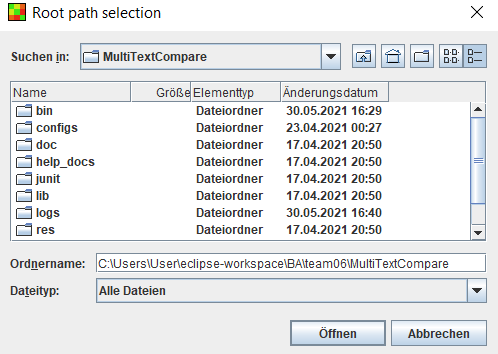
\includegraphics[]{images/metalFileSelection.png}
    \caption{Dateiauswahl unter Metal-\acrshort{lnf}}
    \label{fig:metalFileSelection}
\end{figure}

Als Alternative existieren unter Swing noch weitere, vom Betriebssystem abhängige \acrshort{lnf}s. Diese können mit der Zeile
\begin{minted}{java}
UIManager.setLookAndFeel(UIManager.getSystemLookAndFeelClassName());
\end{minted}
automatisch beim Programmstart geladen und angewandt werden. Zwar ist MultiTextCompare zunächst nur als Windows-Software geplant, allerdings wurde sie bisher immer so entwickelt, dass sie auch auf anderen Betriebssystemen lauffähig ist. Deswegen wird immer das dem Betriebssystem zugehörige \acrshort{lnf} geladen. Die in Abb. \ref{fig:windowsFileSelection} gezeigte Dateiauswahl wirkt dank dem Windows-\acrshort{lnf} nun verständlicher und etwas moderner. Unter Linux würde, sofern es installiert ist, bspw. dann das GTK+ \acrshort{lnf} geladen werden \autocite{lookAndFeel}.

\begin{figure}[!htb]
    \centering
    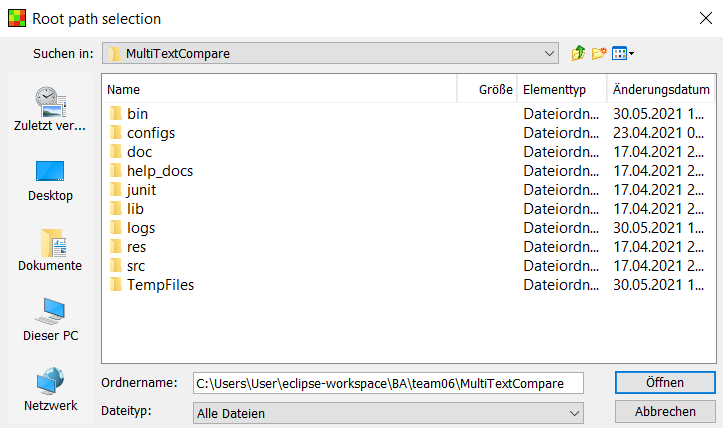
\includegraphics[scale=0.8]{images/windowsFileSelection.png}
    \caption{Dateiauswahl unter Windows-\acrshort{lnf}}
    \label{fig:windowsFileSelection}
\end{figure}

\newpage\subsubsection{Bedienung der Ähnlichkeitsmatrix}

Eine der Anforderungen ist, dass die Software einfach zu bedienen sein soll, jedoch ist die Auswahl der Dateien zur Anzeige der Diff in Version 1.0 in dieser Hinsicht noch nicht optimal. Ein Klick auf eine Zelle innerhalb der Ähnlichkeitsmatrix öffnete eine Diff-Anzeige für die beiden Dateien in der jeweiligen Zeile bzw. Spalte. Um drei Dateien auszuwählen, musste der Benutzer die Spaltenköpfe der Matrix anklicken, was mehrere Probleme beinhaltet. Zum einen musste für jede Datei einzeln die Ähnlichkeit zu anderen Dateien nachgeschaut werden, da die Matrix nicht automatisch die zugehörigen Zellen der ausgewählen Spaltenköpfe gesondert anzeigt. Zum anderen war es nicht möglich nach dem Fund zweier ähnlicher Dateien nach einer dritten ähnlichen Datei zu suchen ohne die ersten beiden immer wieder auszuwählen. Aus diesen Gründen soll das Auswahlsystem komplett überarbeitet werden.

Zunächst sei grundlegend zu erwähnen, dass die Ähnlichkeitsmatrix technisch gesehen eigentlich keine Matrix ist, da diese nicht als Swing-Komponenten existieren. Stattdessen wird eine JTable verwendet, die als erste Spalte Zellen besitzt, die das Aussehen und Verhalten der Spaltenköpfe aus der JTable imitieren. Dies wird durch eine angepasste Version der Klasse \emph{RowNumberTable} von Rob Carrick umgesetzt \autocite{rowNumTable}. Jegliche Funktionen um Klicks des Benutzers innerhalb der Matrix zu bearbeiten basieren also auf den vorgegebenen Funktionen der Klasse JTable. Das Event-Handling dieser Klicks passiert in einer zusätzlichen Handler-Klasse namens \emph{MouseAdapterMatrix}. Diese erbt von der Swing-nativen Klasse \emph{MouseAdapter} und implementiert die Handler-Methode \emph{mousePressed}(), welche das zu handlende Event als Übergabeparameter erhält. 

Praktischerweise lassen sich aus diesem Event die Zeile und Spalte des Klicks auslesen. Da die RowNumberTable die JTable der Matrix einschließt und kein tatsächlicher Teil der klickbaren Matrix ist, verändern sich auch die Indices nicht. 

Um eine Diff-Anzeige zu öffnen soll nun ein Doppelklick notwendig sein, da ein einzelner Klick einfacher zu Fehlklicks führen kann und diese je nach Dateigröße auch eine Wartezeit nach sich ziehen können. Um einen Doppelklick zu erkennen lässt sich die Methode \emph{getClickCount}() auf dem Eventobjekt ausführen. Um drei Dateien auszuwählen, soll nun ein Zwischenschritt eingeführt werden. Zunächst soll es möglich sein eine Zelle als Referenz festzulegen. Dabei werden alle Zellen, die nicht innerhalb der gleichen Zeile und Spalte oder auf der Hauptdiagonale liegen, ausgegraut und sollen damit nicht klickbar sein. Dies führt dazu, dass jeder mögliche Vergleich übersichtlich dargestellt wird und immer genau drei Dateien ausgewählt werden können. Diese Auswahl geschieht dann mit einem weiteren Klick auf eine der farbigen Zelle und führt nicht dazu, dass die Referenzzelle zurückgesetzt wird. Dafür muss der Renderer der JTable wissen, welche Zelle gerade die Referenzzelle ist.

Für solche Fälle existiert eine zentrale Klasse \emph{Management}, die nach dem Singleton-Entwurfsmuster Objekte für sämtliche Klassen instanziiert, von denen genau eine Instanz existieren soll. Zudem können dort Variablen gespeicht werden, die an verschiedenen Stellen im Code gebraucht werden und ebenfalls nur einmal existieren sollten. Beispiele dafür sind die aktuelle Konfiguration der Software oder die eben erwähnte aktuelle Referenzzelle. Für den sog. \emph{TableCellRenderer} wurde die \emph{prepareRenderer}()-Methode so überschrieben, dass sie prüft ob ein boolsches Flag durch die MouseAdapterMatrix im Management gesetzt wurde und dann entweder die Matrix komplett oder nur die Zellen nach den o.\,g. Kriterien koloriert. Das Resultat ist in Abb. \ref{fig:matrixGrau} zu sehen.

\begin{figure}
    \centering
    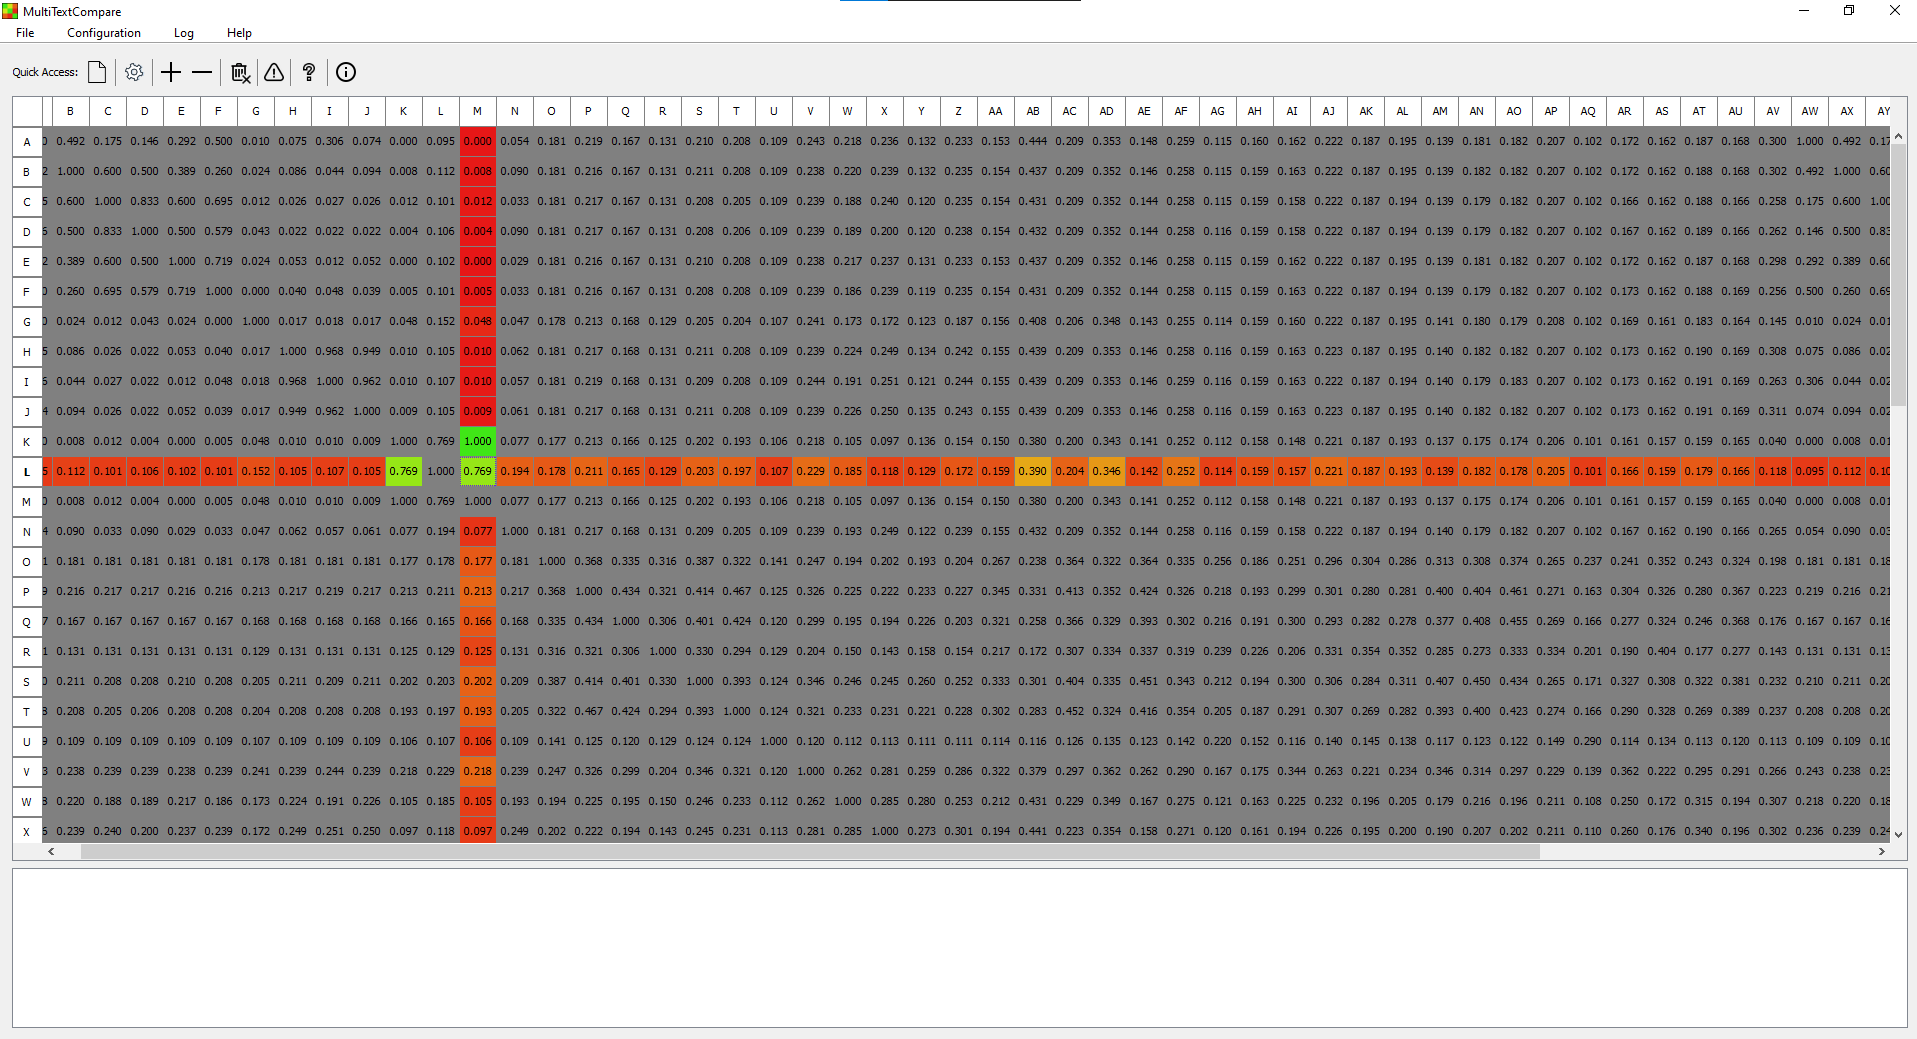
\includegraphics[width=\textwidth]{images/Matrix_neu.png}
    \caption{Ausgrauen der Matrix}
    \label{fig:matrixGrau}
\end{figure}


\subsubsection{Konfiguration}

Im Laufe dieser Arbeit wurden bereits diverse konfigurierbare Parameter besprochen. Darunter fällt u.\,a. die Auswahl der Vergleichsmodi, die Funktionsweise des Matchings, Parameter zum Sortieren oder Normieren der Inputdateien. Zwar erhöht eine größere Anzahl an Konfigurationsparametern die Komplexität der Software für Benutzer und Entwickler, zeitgleich liefert sie aber auch die Möglichkeit die allgemeinen Funktion des Textvergleichs für die zu vergleichenden Dateien anzupassen. Schließlich sind die vorgestellten Vergleichsalgorithmen lediglich Approximationen der Ähnlichkeit von Dateien nach bestimmten Kritierien und bilden daher keine objektive Bewertung für alle möglichen Arten von Wissensrepräsentation innerhalb der unterstützten Dateiformate. Falls der Benutzer Dateien vergleichen möchte, die nicht ideal mit den aktuellen Parametern verglichen werden würden, wäre es sinnvoll mehrere Konfigurationsdateien erstellen zu können und diese einfach auszutauschen anstatt immer wieder die aktuelle Konfiguration zurückzusetzen oder zu überschreiben.

MutliTextCompare erstellt, falls noch nicht vorhanden, eine Standardkonfiguration basierend auf Key-Value Paaren für jeden Parameter. Um eine alternative Konfiguration zu verwenden, wird in der Standardkonfiguration ein weiteres Feld für den Pfad der aktuellen Konfigurationsdatei hinterlegt. Ist dieses nicht leer und die Datei existiert, wird diese Konfiguration verwendet, ansonsten wird die Standardkonfiguration verwendet. Der Benutzer hat dadurch die Möglichkeit die aktuelle Konfiguration über die UI zu überschreiben oder als neue Datei unter Angabe des Dateinamens zu erstellen.

\subsubsection{Persistenz von Vergleichen}

Trotz der bisher durchgeführten Optimierungen für die Vergleiche und das Matching, können Vergleiche mit vielen, großen Dateien durchaus noch einige Minuten dauern. Solche langen Wartezeiten können sehr unangenehm sein, besonders wenn die gleichen Vergleichsergebnisse zu einem späteren Zeitpunkt wieder gebraucht werden. Es ist allerdings in Java bspw. durch Serialisierung möglich, bestimmte Programmteile persistent zu speichern. 

Nach Erstellung und Anzeige der Ähnlichkeitsmatrix wird die Diff für Dateien erst berechnet, wenn sie vom Benutzer ausgewählt wurden. Falls vergleichsbezogene Parameter geändert werden, muss die Matrix neu berechnet werden, um diese zu sehen. Das heißt, dass es ausreicht genau den Programmzustand wiederherzustellen, bei dem die Matrix gerade erzeugt wurde. Innerhalb des Codes wird dafür die Liste mit den berechneten Vergleichen der Matrix benötigt. Zusätzlich muss die Map der \emph{FileImporter}-Komponente gespeichert werden, die die erstellten temporären Dateien auf die Originaldateien mappt. Letztlich wird eine geordnete Liste der ausgewählten Dateien  bzw. ihrer Dateipfade mit zugehörigem Index gespeichtert. Zwar könnte diese Liste aus der Map wiederhergestellt werden, allerdings müssten dafür einige Methoden zentralisiert oder publik gemacht werden, was die Abhängigkeiten der Klassen und damit die Komplexität der Code-Base weiter erhöht.

Für die persistente Speicherung über Serialisierung muss sichergestellt werden, dass alle zu speichernden Objekte das Interface \emph{Serializable} implementieren. Dies muss nur für die selbst erstellte Matrix bzw. die Klasse \emph{ICompareImpl} nachgeholt werden. Um die Objekte zu serialisieren wird die native Java Klasse \emph{ObjectOutputStream} verwendet und mit einem \emph{FileOutputStream} in eine Datei geschrieben. Der Dateiname ist vom Benutzer wählbar und besitzt immer die Dateiendung \emph{.mtc}. Damit die Objekte korrekt ein- und ausgelesen werden können, müssen diese in der gleichen Reihenfolge geschrieben und gelesen werden.

Da die Map des FileImporters nur Referenzen auf die Dateien enthält, muss noch sichergestellt werden dass die temporären Dateien eines Vergleichs mitgespeichert werden um die an den Dateien vorgenommenen Normierungen und Sortierungen korrekt anzuzeigen. Dafür wird für jeden gespeicherten Vergleich ein Verzeichnis erstellt, indem sowohl die mtc-Datei mit den gespeicherten Objekten, als auch ein Verzeichnis mit den zugehörigen temporären Dateien vorliegt. Diese temporären Dateien werden dann in das \emph{TempFiles}-Verzeichnis der Software kopiert sobald der jeweilige Vergleich geladen wurde.

\subsubsection{Benutzerfeedback und Logging}\label{logging}

Beim Öffnen von MultiTextCompare erscheint in der unteren Hälfte des Panels ein Log. Dieser dient dazu, dem Benutzer Feedback zu seinen Aktionen zu liefern, bspw. wenn eine Referenzzelle bei der Auswahl von Dateien für die Diff-Anzeige selektiert wird. Zusätzlich werden so Fehler beim Parsen oder interne Fehler während der Laufzeit an den Benutzer weitergegeben. Bisher gab es jedoch keine Unterscheidung nach der Schwere des Fehlers oder der Wichtigkeit der Nachricht, was durch eine interne Logging-Komponente geändert werden soll. Wie bereits im Kapitel zu Architektur in \ref{architektur} gezeigt wurde, funktioniert diese Logging-Komponente außerhalb der eigentlichen 3-Schichten-Architektur. 

Es existiert zwar im Paket \emph{java.util.logging} bereits eine native Logging-Lösung, aber sie ist hier fast schon zu umfangreich und benötige mehr Arbeit um sie in die Code-Base einzupflegen. In der eigenen Logger-Komponenete werden nur 3 Log-Level unterschieden: 
\begin{description}
\item[Info] Beinhaltet das Feedback zur User-Interaktion und Benachrichtigungen über Berechnungen wie den Beginn des Vergleichs und das Ende mit der Berechnungsdauer. Hier handelt es sich um optionale Ausgaben, die besonders dann signifikant sind, wenn eine Berechnung länger dauert oder sich der Benutzer bei der Bedienung der Software noch nicht sicher ist. Diese Ausgaben werden als regulärer Text im Log hinterlegt.

\item[Warning] Bei diesem Level werden Fehler aufgeführt die entweder durch falsche Benutzung der Software auftreten oder durch fehlerhafte Inputdateien. Ein Beispiel für falsche Benutzung wäre z.\,B. der Versuch einen Vergleich persistent zu speichern bevor überhaupt eine Matrix erzeugt wurde. Warnings führen nicht zu Fehlverhalten und werden mit roter Schrift auf gelbem Hintergrund im Log angezeigt.

\item[Error] Errors sind schwerwiegende Fehler, die dazu führen dass das Programm nicht ordnungsgemäß funktionieren kann. Der wahrscheinlichste Fehler auf diesem Level ist eine \emph{FileNotFoundException}, die geworfen wird falls Dateien unerwartet gelöscht, verschoben oder umbenannt wurden. Diese Fehler werden im Log mit rotem Hintergrund und weißer Schrift angezeigt.
\end{description}

Zusätzlich zur Anzeige im Log werden diese Ausgaben auch persistent in Logdateien gespeichert. Um riesige Logdateien und damit einen Verlust der Übersicht zu vermeiden, werden die Logs nach Datum getrennt. Für jede Logausgabe wird dafür geprüft ob eine aktuelle Logdatei existiert, ansonsten wird eine neue Datei erstellt. Zwar werden alle Logausgaben unabhängig vom Level in die Logdateien geschrieben, dem Benutzer ist es aber möglich einzelne Level für die Anzeige im Log ein- und auszuschalten.

  \section{Test und Auswertung}\label{test}

Das letzte Kapitel des Hauptteils soll nun die wichtigsten Verbesserungen aus Kapitel \ref{implementierung} im Anwendungskontext zeigen und evaluieren.

\subsection{Übersicht der Testsysteme}

Zunächst sollen die Testsysteme vorgestellt werden. Es geht bei der Analyse der Laufzeit hierbei nicht darum, die Hardwarekonfigurationen untereinander zu vergleichen, sondern um die Darstellung der durch das Batch-Processing eingeführten Skalierbarkeit. PC1 ist dabei der schnellste PC, gefolgt von PC2 und PC3, wobei letzterer der Konfiguration der Laborrechner am meisten ähnelt. Das in der Tabelle angegebene Jahr bezieht sich auf das Einführungsdatum der jeweiligen CPU, die den größten Einfluss auf die Berechnungsdauer hat. 

Auf allen Computern ist Windows 10 in einer 64 Bit Version installiert. Außerdem wird Java sowohl beim \acrshort{jdk}, als auch bei der \acrshort{jre} in der 32 Bit Variante unter Version 1.7.0\_75 verwendet. Desweiteren wird MultiTextCompare immer über Eclipse selbst und nicht über eine ausführbare \acrshort{jar} gestartet. Um eine vollständige Auslastung der CPU sicherzustellen werden die Run Commands für das Programm so angepasst, dass bis zu 1 GB RAM verwendet werden kann. Zusätzlich werden die Vergleiche direkt nach dem Start der PCs ausgeführt ohne dass weitere Programme geöffnet werden.
\begin{table}[!htb]
\centering
\begin{tabular}{|l||l|l|l|}
\hline
Hardwarekomponente & PC1      & PC2      & PC3      \\ \hline
CPU &
  \begin{tabular}[c]{@{}l@{}}Intel i9 10850k\\ (10c/20t)\end{tabular} &
  \begin{tabular}[c]{@{}l@{}}Intel i7 7700HQ\\ (4c/8t)\end{tabular} &
  \begin{tabular}[c]{@{}l@{}}Intel i5 4570\\ (4c/4t)\end{tabular} \\
  \hline
RAM &
  \begin{tabular}[c]{@{}l@{}}32GB DDR4 \\ @ 2933 MHz\end{tabular} &
  \begin{tabular}[c]{@{}l@{}}8GB DDR4\\ @ 2400 MHz\end{tabular} &
  \begin{tabular}[c]{@{}l@{}}16GB DDR3\\ @ 1600 MHz\end{tabular} \\
  \hline
Festplatte         & NVMe SSD & NVMe SSD & SATA SSD \\ \hline
Jahr \autocite{intelSpec}    & 2020 & 2017 & 2013 \\ \hline
\end{tabular}
\caption{Hardwarekonfigurationen der Testsysteme}
\label{table:hardware}
\end{table}

\subsection{Laufzeitoptimierung durch Multithreading}

Als erstes soll das Laufzeitverhalten beim Aufbau der Matrix untersucht werden. Dadurch dass MultiTextCompare aber für beliebige textbasierte Dateien konzipiert ist, lässt sich hier allerdings kein \glqq typischer\grqq{} Fall herstellen, da die Laufzeit sehr stark von den verglichenen Dateien und den Konfigurationsparametern abhängt. Deshalb soll hier nur erfasst werden, wie groß die Zeitersparnis im \emph{best case} ist.

Für den ersten Durchlauf werden 80 reguläre Textdateien erstellt, deren Inhalt identisch ist. Beim Inhalt wird der Platzhaltertext \emph{Lorem ipsum} verwendet, welcher über den Line Compare-Vergleichsmodus ohne Zeilenmatching verglichen wird. Die Dateien sind 196KB groß, besitzen 611 Zeilen und die Zeichen pro Zeile variieren ca. zwischen 100 und 1700. Gemessen wird die Dauer des Vergleichs mit und ohne Multithreading und der Overhead, der durch das Verteilen und Zusammenfügen der gewichteten Vergleiche zusätzlich aufkommt. Dafür wird im Code mittels 
\begin{minted}{java}
System.nanoTime()
\end{minted}

der Start- bzw. Endzeitpunkt der Messung festgehalten und die Differenz der beiden Werte als Ergebnis notiert. Da \acrshort{io}-Zugriffe und das Scheduling des Betriebssystems Varianzen in die Laufzeit einbringen, werden die Ergebnisse bei einer Dauer von unter fünf Minuten über fünf Durchläufe gemittelt.

\begin{table}[!htb]
\centering
\begin{tabular}{|l|c|c|c|}
\hline
Testlauf            & PC1 & PC2 & PC3 \\ \hline
Ohne Multithreading & 43min 11s  & 66min 29s  & 68min 37s  \\ \hline
Mit Multithreading  & 4min 26s  & 20min 49s  & 18min 27s  \\ \hline
Overhead            & 2,355s  & 6,241s  & 2,440s  \\ \hline
\end{tabular}

\caption{Messergebnisse für Multithreading}
\label{table:multithreading}
\end{table}

Die Messergebnisse sind in Tabelle \ref{table:multithreading} dargestellt und zeigen wie erwartet, dass die Vergleiche ohne Multithreading auf PC1 am schnellsten und auf PC3 am langsamsten durchlaufen. Mit Multithreading ist PC3 aber schneller als PC2, was wahrscheinlich der besseren Kühlleistung des Systems geschuldet ist. Der Unterschied zwischen Vergleichen die multi- bzw. single-threaded sind ist zwar erheblich, allerdings korrespondiert dieser nicht unbedingt genau mit der Anzahl der verfügbaren Prozessorkerne. Bei PC1 mit zehn Prozessorkernen, ist eine Verbesserung um ungefähr den gleichen Faktor erkennbar. PC2 hat mit 4 physischen Kernen aber nur knapp eine Verbesserung um den Faktor 3,3. Da sich die einzelnen Prozessoren auch in der Leistung, z.B. der Taktrate oder der Instruktionen pro Takt, unterscheiden, sind erhebliche Unterschiede ohne Multithreading erkennbar. 

Auch der entstandene Overhead durch die Verteilung und das Zusammenführen der Batches variiert zwischen den Systemen merkbar. Dieser Wert ist aber wenig signifikant wenn die mögliche Zeitersparnis durch das Multithreading betrachtet wird. Am meisten Zeit verbraucht dabei die Gewichtung der Vergleiche, für die alle Dateien der Vergleiche eingelesen werden müssen. Faktoren für die Abweichungen zwischen den Systemen können hier auch die Leistung der CPU, der Festplatten und das Scheduling des Betriebssystems sein, da keins der Systeme identische Komponenten beinhaltet. 

Mit Multithreading entsteht also eine große Zeitersparnis, wenn die Systeme die nötige Hardware bieten. Hier gibt es aber auch noch weitere Möglichkeiten um die Wartezeit für den Benutzer zu verringern. Für zwei Zeilen mit vielen Zeichen entsteht bspw. das Problem, dass die Berechnung der Levenshtein-Distanz dort relativ teuer wird. Dort könnte es sinnvoll sein, die Strings in kleinere Sequenzen zu zerlegen und diese zu vergleichen. Ansonsten kann aber auch konfiguriert werden, dass Zeilen nur bis zu einer bestimmten Edit Distance verglichen werden und bei einer Überschreitung mit der Ähnlichkeit 0 bewertet werden. 

\subsection{Strukturbasierte Vergleichsmodi}

Die beiden neu eingeführten Vergleichsmodi für XML und JSON können für bestimmte Anwendungsfälle die Ähnlichkeitsbewertung von Dateien deutlich hinsichtlich ihrer Präzision verbessern. Da Knoten nur verglichen werden falls ihre eindeutigen Identifier übereinstimmen, sind false positives deutlich unwahrscheinlicher als bspw. beim Modus Line Compare, bei dem nicht gematchte Zeilen trotzdem miteinander verglichen werden und eine zufällige, wenn auch geringe, Ähnlichkeit haben können. Dadurch werden weniger, aber dafür tatsächlich strukturell ähnlichere Dateien in der Matrix als Ähnlich dargestellt und vor einer möglichen Auswahl der Diff gefiltert. Ein weiterer Vorteil kann im Bereich der Laufzeit entstehen, da ganze Teilbäume aufgrund von unterschiedlichen Bezeichnern evtl. nicht verglichen werden müssen. 

Im Folgenden soll der strukturbasierte Vergleich für Dateien des Typs JSON angewandt und mit den Ergebnissen des Modus Line Compare verglichen werden. Dafür werden drei Beispielkonfigurationen einer fiktiven Rest-Schnittstelle verwendet, bei denen es sich um unterschiedliche Versionen handelt. Diese Konfigurationsdateien sind in Abb.\ref{fig:structCompJson} dargestellt und zwecks Übersicht relativ einfach gehalten. Datei V0 enthält die wenigsten Funktionalitäten, denn es fehlt im Vergleich zu V1 bspw. die Authentifizierung des zugreifenden Akteurs oder die Validierung der übergebenen JSON- oder XML-Inhalte. Der Unterschied von V1 zu V2 ist dafür deutlich kleiner, es ändert sich lediglich der Host von einer IP-Adresse zu einem tatsächlichen Domain-Namen und es kommt ein weiteres Dateiformat in Form von YAML für schreibende Anfragen dazu. 

\begin{figure}[!htb]
\centering
\begin{subfigure}[t]{.45\textwidth}
  \begin{minted}[stripnl=false, fontsize=\small]{json}
{
    "api_version" : "v0",
    "endpoint" : {
        "host" : "192.168.0.165",
        "port": 5000
    },
    "accept_format": [
        "xml",
        "json"
    ],
    "request_types": [
        "GET",
        "POST",
        "PUT",
        "DELETE"
    ]
}
 
 

 
 
  \end{minted}
  \caption{Konfiguration V0}
  \label{fig:sub1}
\end{subfigure}
\begin{subfigure}[t]{.45\textwidth}
\begin{minted}[stripnl=false, fontsize=\small]{json}
{
    "api_version" : "v1",
    "endpoint" : {
        "host" : "201.177.6.52",
        "port": 5000
    },
    "accept_format": [
        "xml",
        "json"
    ],
    "authentication": {
        "user": "$username",
        "pass": "$password"
    },
    "enable_validation": true,
    "request_types": [
        "GET",
        "POST",
        "PUT",
        "DELETE"
    ]
}
\end{minted}
  \caption{Konfiguration V1}
  \label{fig:sub2}
\end{subfigure}
\begin{subfigure}{.45\textwidth}
\begin{minted}[stripnl=false, fontsize=\small]{json}

{
  "api_version": "v2",
  "endpoint": {
    "host": "test@server.de",
    "port": 5000
  },
  "accept_format": ["xml", "json", "yaml"],
  "authentication": {
    "user": "$username",
    "pass": "$password"
  },
  "enable_validation": true,
  "request_types": [
        "GET",
        "POST",
        "PUT",
        "DELETE"
    ]
}

\end{minted}
  \caption{Konfiguration V2}
  \label{fig:sub2}
\end{subfigure}
\caption{Testdateien für strukturbasierten Vergleich}
\label{fig:structCompJson}
\end{figure}


Beim strukturellen Vergleich werden nun zunächst die entsprechenden Dokumentbäume aufgestellt. Die maximale Anzahl an Knoten auf Ebene 1 beträgt sechs. Jeder dieser Knoten geht also für seinen Inhalt mit einem Gewicht von $\frac{1}{6}$ in die Gesamtähnlichkeit ein. Beim zeilenbasierten Vergleich ist hingegen die maximale Anzahl an Zeilen für das Gewicht entscheidend. Aus Platzgründen wurde die Darstellung der \emph{request\_types} in Abb. \ref{fig:structCompJson} mit einem Array-Eintrag pro Zeile gewählt, der JSON-Parser von Jackson schreibt allerdings das gesamte Array in eine Zeile weswegen sich eine maximale Zeilenanzahl von 14 und damit ein Gewicht von $\frac{1}{14}$ pro Zeile ergibt. Das heißt hier für die Bewertung, dass beim Vergleich von V0 und V1 die fehlende Authentifizierung im strukturellen Vergleich $\frac{1}{6}$ und im zeilenbasierten Vergleich $\frac{4}{14}$ der Gesamtähnlichkeit kostet. Dieser Effekt entsteht, da der zeilenbasierte Modus nicht auf die Struktur von JSON bzw. auch auf die Darstellung von JSON-Dateien durch den Parser achten kann. Die Ergebnisse aller Vergleiche sind in Tabelle \ref{table:vergleichsmodi} dargestellt. 

\begin{table}[!htb]
    \setlength{\tabcolsep}{8pt}
    \begin{subtable}{.5\linewidth}
      \centering
        \begin{tabular}{|l|c|c|c|}
        \hline
        Ähnlichkeit            & V0 & V1 & V2 \\ \hline
        V0 & 1,000  & 0,526  & 0,444  \\ \hline
        V1  & 0,526  & 1,000  & 0,784  \\ \hline
        V2 & 0,444  & 0,784  & 1,000  \\ \hline
        \end{tabular}
        \caption{struktureller Vergleich}
    \end{subtable}%
    \begin{subtable}{.5\linewidth}
      \centering
        \begin{tabular}{|l|c|c|c|}
        \hline
        Ähnlichkeit            & V0 & V1 & V2 \\ \hline
        V0 & 1,000  & 0,618  & 0,594  \\ \hline
        V1  & 0,618  & 1,000  & 0,954  \\ \hline
        V2 & 0,594  & 0,954  & 1,000  \\ \hline
        \end{tabular}
        \caption{zeilenbasierter Vergleich}
    \end{subtable} 
    \caption{Vergleichsergebnisse für die Dateien aus Abb. \ref{fig:structCompJson}}
    \label{table:vergleichsmodi}
\end{table}

Aus den Ergebnissen wird deutlich, dass die Vergleichsmodi die Ähnlichkeit zwar unterschiedlich, dafür aber ohne Widersprüche bewerten. Der Vergleich von V1 und V2 ist bei beiden Modi der ähnlichste, es folgen V1 und V0 und zuletzt kommen V0 und V2. Letzteres ist dadurch erklärbar, dass in V0 und V1 im Feld \emph{host} noch IP-Adressen stehen, die durch die Trennpunkte und die in beiden Adressen vorkommenden Zahlen eine höhere Ähnlichkeit haben als eine Adresse und ein Domain-Name.
Der Hauptunterschied liegt also weniger in der Richtung der Bewertung, also ob der Wert näher an 0 oder näher an 1 ist, sondern in den absoluten Werten. Besonders die hohe Ähnlichkeit beim Vergleich von V1 und V2 ist beim zeilenbasierten Vergleich dadurch entstanden, dass die identischen Attributschlüssel eine Grundähnlichkeit für die Zeilen herstellen in denen sie vorkommen. Ebenfalls erhöht die identische Struktur die Ähnlichkeit, da Markup wie Klammern und Kommata in den gleichen Zeilen liegen und somit die Ähnlichkeit um bis zu $\frac{1}{14}$ anheben. Hier kommen also die Vorteile des strukturbasierten Modus zum tragen, bei dem Markup nicht für die Ähnlichkeit berücksichtigt wird und ausschließlich der Inhalt der Dateien bewertet wird. 

In Tabelle \ref{table:structCompDiff} sind die Abzüge in der Ähnlichkeit für den Vergleich von V1 zu V2 dargestellt. Drei der Key-Value-Paare sind identisch und werden deshalb nicht aufgelistet. Für den Schlüssel \emph{api\_version} existieren zwei Zeichen und eins davon unterscheidet sich, wodurch ein erster Abzug von $\frac{1}{12}$ entsteht. Das Objekt \emph{endpoint} hat ein identisches Paar für den Port, nur der Hostname unterscheidet sich. Da die Hostnamen mit dem Punkt nur ein gemeinsames Zeichen haben, kommt hier ein großer Unterschied zu stande. Die 0,464 aus der Tabelle wird durch \[ \frac{1}{2} - \Big(\frac{1}{2} \cdot \big(1 -  \frac{13}{14}\big) \Big) = 0,464 \] errechnet und beschreibt den Unterschied der \emph{endpoint}-Objekte zwischen den beiden Dateien. In der Formel wird letztendlich nur die gewichtete Ähnlichkeit der Hostnamen von der Ähnlichkeit der Ports subtrahiert. Im Array \emph{accept\_format} fehlt in V1 noch der Eintrag für YAML und führt zu einem Abzug von $\frac{1}{3}$ im Kontext des Feldes bzw. $\frac{1}{18}$ im Kontext der Gesamtähnlichkeit. Werden nun alle Abzüge von der maximalen Ähnlichkeit 1 subtrahiert, entsteht der Wert aus Tabelle \ref{table:vergleichsmodi}(a) für den Vergleich von Datei V1 und V2.

\begin{table}[]
\centering
\begin{tabular}{|l|c|}
\hline
Attributschlüssel   & Abzug \\ \hline
api\_version          & \large$ \frac{1}{6} \cdot \frac{1}{2} = \frac{1}{12} $ \\ \hline
endpoint             & \large$ \frac{1}{6} \, \cdot \, $\small $ 0,464 \approx 0,077 $ \\ \hline
accept\_format       & \large$ \frac{1}{6} \cdot \frac{1}{3} = \frac{1}{18} $  \\ \hline
\end{tabular}



\caption{Bewertung der inhaltlichen Unterschiede für V1 und V2}
\label{table:structCompDiff}
\end{table}

Es sei allerdings noch abschließend zu erwähnen, dass die hier gezeigten Dateien nur einen Anwendungsfall abdecken. Die Anwendung ist zwar nicht für einen bestimmten Anwendungsfall konzipiert, es kann im Rahmen dieser Arbeit aber nicht jeder mögliche Fall dargestellt und analysiert werden. 

  \section{Zusammenfassung und Ausblick}

Im Rahmen dieser Arbeit wurde eine bereits existierende Software zum Vergleich von beliebig vielen textbasierten Dateien überarbeitet und erweitert. Besonders im Fokus standen die Aspekte der Genauigkeit von Algorithmen, der Laufzeit, sowie der Benutzbarkeit und Verständlichkeit der Anwendung. Dafür wurde zunächst das Zeilenmatching in der bestehenden Funktionsweise untersucht, wobei nennenswerte funktionale und zeitliche Verbesserungen bspw. durch das neue \emph{Best Match}-Verfahren eingeführt werden konnten. Ähnliches galt auch für den zeilenweisen Textvergleich, dessen Funktionsweise durch die Integration der Matching-Komponente hinsichtlich der Genauigkeit verbessert wurden. Zusätzlich profitiert der Vergleichsmodus nun von den zuvor genannten Verbesserungen des Zeilenmatchings. 

Ein weiterer großer Teil der Arbeit bestand daraus, zwei neue Vergleichsalgorithmen für XML und JSON zu konzipieren und zu implementieren. Diese arbeiten primär auf einer strukturellen Basis mit Hilfe von Dokumentbäumen und sind in der Lage Markup zu ignorieren und daher strikt inhaltlich zu vergleichen. Da die Algorithmen Elemente größtenteils anhand von eindeutigen Identifiern matchen und vergleichen, sind sowohl semantisch genauere als auch insgesamt schnellere Vergleiche möglich. Letzteres entsteht dadurch, dass ganze Teilbäume vom Vergleich ausgeschlossen werden können, wenn der zugehörige Identifier nur in einer Datei existiert. Zusätzlich eliminieren die Algorithmen durch dieses Vorgehen die Möglichkeit von zufälligen, falschen Bewertungen.

In Hinblick auf die Laufzeit wurde ein Verfahren entwickelt, womit die Anwendung verfügbare Hardware effektiv nutzt. Vergleiche werden nun gleichmäßig auf verfügbare CPU-Threads verteilt, wodurch für jeden Vergleichsmodus je nach Hardwarekonfiguration proportionale Verbesserungen messbar sind. Sowohl die Laufzeitverbesserungen als auch die Funktionsweise der strukturbasierten Algorithmen wurden zudem in Kapitel \ref{test} anhand von Beispieldateien präsentiert.

Auch das User Interface erhielt zahlreiche Änderungen, die sowohl kosmetisch als auch funktional sind. Neben einer Änderung des Java-spezifischen \emph{Look-and-Feels}, welches nun abhängig vom unterliegenden Betriebssystem ist, wurden weitere Funktionen erstellt um die Benutzung der Software für den Benutzer angenehmer zu machen. Die Auswahl von Dateien für eine graphische Anzeige der Unterschiede gibt dem Benutzer nun durch das Ausgrauen der Matrix zusätzliche visuelle Informationen dazu, welche Vergleiche sinnvoll auszuwerten wären. Zudem können Vergleiche nun persistent gespeichert werden, die Funktionsweise kann durch mehr Parameter für den vorliegenden Anwendungsfall angepasst werden und Aktionen und Fehler werden nun automatisch über ein eigenes Log-System festgehalten.

Insgesamt lässt sich sagen, dass die Anwendung MultiTextCompare sich nun nicht mehr nur durch die Anzahl der zu vergleichenden Dateien von bestehender Software abhebt, sondern zusätzlich Möglichkeiten bietet um Dateien vom Typ JSON und XML spezialisiert inhaltlich zu vergleichen. 

Trotzdem gibt es noch Aspekte, die verbessert werden können. Dazu zählt z.B. eine weitere Anpassung im Matching, die nicht mehr bloß zeilenbasiert nach Matches sucht, sondern tatsächlich versucht verschobene Textblöcke zu erstellen. Desweiteren könnte die Matching-Komponente auch auf XML und JSON angepasst werden, sodass diese auch Markup erkennt und diesen beim Feststellen von Matches besonders beachtet. Dies ist auch etwas was in Abb. \ref{fig:bestMatchResult} zu sehen war, wo Markup-Elemente gleichermaßen zur Ähnlichkeit von Zeilen beigetragen haben wie der eigentliche Inhalt der Dateien. Das Best-Match Verfahren bringt zwar bessere Ergebnisse als wenn nach dem erstem Match die Suche abgebrochen wird, aber die Darstellung könnte durch eine Spezialisierung auf bestimmte Dateiformate weiter verbessert werden. Als letzten Punkt ließe sich noch die Einbindung des Dateiformats YAML nennen. Dies ist besonders im in der Einleitung genannten Cloud-Umfeld als Konfigurationsformat weit verbreitet und ist auch durch die Jackson Bibliothek unterstützt. Da JSON eine direkte Untermenge von YAML ist \cite{yamlSpec}, sollte auch der strukturelle Vergleichsalgorithmus nicht neu entwickelt, sondern bloß angepasst werden müssen.
  % INFO: Querverweise auf Gliederungselemente, Abbildungen 
  %       & Tabellen setzen:
  %
  % Voraussetzung: Gesetzte Referenzmarke mit dem Befehl: \label{marke}
  % 
  % Referenzierung erfolgt dann mittels dem Befehl:
  % \ref{marke}
  
  \newpage 

  % Literaturverzeichnis
   % INFO: Referenzieren auf das Literaturverzeichnis:
   %
   % Befehl: \cite{refmarke}
   % 
   % "refmarke" ist die Angabe in den geschweiften Klammern bei 
   % \bibitem[]{refmarke}. 
   \newpage
    \thispagestyle{empty}
\section{Quellenverzeichnis}
  \printbibliography[heading=none]

  
  % INFO: Biblatex -Ausgabe des  
  % Literaturverzeichnisses (Beispiele):   
  % - \printbibliography => Ausgabe ALLER 
  %   Einträge
  % - \printbibliography[nottype=online]
  %   => Ausgabe der Einträge, bis auf die
  %      "Online"-Einträge
  % - \printbibliography[type=online]     
  %   => Ausgabe nur der "Online"-Einträge  
   %\printbibliography

  % Anhang
  \newpage
  \setcounter{section}{0} % Nummerierung der Gliederungsebene "section" auf 0 setzen
  \renewcommand*\thesection{\Alph{section}} % Nummerierungsart für die Gliederungsebene "section" 
  % auf Großbuchstaben setzen
 % \section{Anhang}\label{anhang}
 %  \subsection{Unterabschnitt von Anhang}\label{subsec_UabsAnhang}
 %  TEXT FOLGT...
  
  \newpage
  
 % Erklärung über die selbständige Abfassung der Arbeit  
 \pagestyle{empty}
 \section*{Erklärung über die selbständige\\Abfassung der Arbeit} % \section*{...}: das *-Symbol erlaubt, dass dieser
 % Gliederungspunkt nicht ins Inhaltsverzeichnis aufgenommen wird
 \addcontentsline{toc}{section}{Erklärung über die selbständige Abfassung der Arbeit}
 Ich erkläre an Eides statt, dass ich die vorgelegte Abschlussarbeit selbständig und
 ohne fremde Hilfe verfasst, andere als die angegebenen Quellen und Hilfsmittel
 nicht benutzt und die den benutzten Quellen wörtlich oder inhaltlich entnommenen
 Stellen als solche kenntlich gemacht habe.\\\\
\begin{tabular}{cp{7cm}}
    & \\ 
    & \\ \hline
  \small (Ort, Datum, Unterschrift) & \normalsize \\
  \end{tabular} 
   
\newpage
% Unbeschriftetes Abschlussblatt (Leere Seite)
\thispagestyle{empty}
\section*{}  
          
    
\end{document}

